%%%%%%%%%%%%%%%%%%%%%%%%%%%%%%%%%%%%%%%%%%%%%%%%%%%%%%%%%%%%%%%%%%%%%%%
%%%%%%%%%%%%%%%%%%%%%%%%%%%%%%%%%%%%%%%%%%%%%%%%%%%%%%%%%%%%%%%%%%%%%%%
%%%%%                                                                 %
%%%%%     report.tex                                                  %
%%%%%                                                                 %
%%%%% Author:      Florian Zaruba                                     %
%%%%% Created:     10.12.2015                                         %
%%%%% Description: Report for PULPino and Imperio architecture        %
%%%%%                                                                 %
%%%%%%%%%%%%%%%%%%%%%%%%%%%%%%%%%%%%%%%%%%%%%%%%%%%%%%%%%%%%%%%%%%%%%%%
%%%%%%%%%%%%%%%%%%%%%%%%%%%%%%%%%%%%%%%%%%%%%%%%%%%%%%%%%%%%%%%%%%%%%%%

%%%%%%%%%%%%%%%%%%%%%%%%%%%%%%%%%%%%%%%%%%%%%%%%%%%%%%%%%%%%%%%%%%%%%%%
%%%%%                                                                 %
%%%%%     Document Class                                              %
%%%%%                                                                 %
%%%%%%%%%%%%%%%%%%%%%%%%%%%%%%%%%%%%%%%%%%%%%%%%%%%%%%%%%%%%%%%%%%%%%%%
\documentclass[%
 oneside,      % Use the same margins for odd and even pages (cannot
               % be used with the 'twoside' option).
% twoside,      % Use different margins for odd and even pages (cannot
               % be used with the 'oneside' option).
 openany,      % Open chapters on odd and even pages.
 halfparskip,  % Create small spaces for new paragraphs but no indents.
]{scrbook}

%%%%%%%%%%%%%%%%%%%%%%%%%%%%%%%%%%%%%%%%%%%%%%%%%%%%%%%%%%%%%%%%%%%%%%%
%%%%%                                                                 %
%%%%%     Preamble                                                    %
%%%%%                                                                 %
%%%%%%%%%%%%%%%%%%%%%%%%%%%%%%%%%%%%%%%%%%%%%%%%%%%%%%%%%%%%%%%%%%%%%%%
% Load the preamble from another file.
%%%%%%%%%%%%%%%%%%%%%%%%%%%%%%%%%%%%%%%%%%%%%%%%%%%%%%%%%%%%%%%%%%%%%%%
%%%%%%%%%%%%%%%%%%%%%%%%%%%%%%%%%%%%%%%%%%%%%%%%%%%%%%%%%%%%%%%%%%%%%%%
%%%%%                                                                 %
%%%%%     preamble.tex                                                %
%%%%%                                                                 %
%%%%% Author:      Florian Zaruba                                     %
%%%%% Created:     10.12.2015                                         %
%%%%% Description: Report for PULPino and Imperio architecture        %
%%%%%                                                                 %
%%%%%%%%%%%%%%%%%%%%%%%%%%%%%%%%%%%%%%%%%%%%%%%%%%%%%%%%%%%%%%%%%%%%%%%
%%%%%%%%%%%%%%%%%%%%%%%%%%%%%%%%%%%%%%%%%%%%%%%%%%%%%%%%%%%%%%%%%%%%%%%


%%%%%%%%%%%%%%%%%%%%%%%%%%%%%%%%%%%%%%%%%%%%%%%%%%%%%%%%%%%%%%%%%%%%%%%
%%%%%                                                                 %
%%%%%     Package Loading                                             %
%%%%%                                                                 %
%%%%%%%%%%%%%%%%%%%%%%%%%%%%%%%%%%%%%%%%%%%%%%%%%%%%%%%%%%%%%%%%%%%%%%%

% Determines the input encoding.
\usepackage[%
 utf8,
% latin1
]{inputenc}

% ---------------------------------------------------------------------

% Determines the output encoding.
\usepackage[T1]{fontenc}

% ---------------------------------------------------------------------

% Determines language settings.
\usepackage[%
 english    % You may change this to 'ngerman' in order to write a
            % german report.
]{babel}

% ---------------------------------------------------------------------

% Provides image loading.
\usepackage{graphicx}

% ---------------------------------------------------------------------

% Provides customization of chapter headings.
\usepackage[%
	Lenny     % Choose a nice layout for chapter headings.
]{fncychap}

% ---------------------------------------------------------------------

% Provides some blindtext.
\usepackage{lipsum}

% ---------------------------------------------------------------------

% Provides stretchable tables.
\usepackage{tabularx}

% ---------------------------------------------------------------------

% Provides some fancy boxes.
\usepackage{fancybox}

% ---------------------------------------------------------------------

% Provides subfigures.
\usepackage{subfig}

% ---------------------------------------------------------------------

% Provides colors in LaTeX.
\usepackage{xcolor}

% ---------------------------------------------------------------------

% Provides conditionals (for titlepage).
\usepackage{xifthen}

% ---------------------------------------------------------------------

% Provides the algorithm environment
\usepackage[ruled,%
            linesnumbered]{algorithm2e}

% ---------------------------------------------------------------------

% Provides bold greek math symbols.
\usepackage{bm}

% ---------------------------------------------------------------------

% Allows to include pdf documents.
\usepackage{pdfpages}

% ---------------------------------------------------------------------

% Provides nicer tables than the standard tables.
\usepackage{booktabs}

% ---------------------------------------------------------------------

% Provides simple line spacings.
\usepackage{setspace}

% ---------------------------------------------------------------------

% Provides simple line spacings.
\usepackage{geometry}

% ---------------------------------------------------------------------

% Provides more customizeable captions.
\usepackage{capt-of}

% ---------------------------------------------------------------------

% Provides small table of contents (e.g., for single chapters or the
% appendix).
\usepackage{minitoc}

% ---------------------------------------------------------------------

% Provides a simple command to describe a directory tree.
\usepackage{dirtree}

% ---------------------------------------------------------------------

%%%%%                                                             %%%%%
%%%%% ATTENTION: Loading further packagaes should go in here.     %%%%%
%%%%%                                                             %%%%%

\usepackage{listings}
\usepackage{bytefield}

% ---------------------------------------------------------------------

% Provides hyperlinks within your document. Should always be loaded at
% the end.
\usepackage{hyperref}

% ---------------------------------------------------------------------

% Provides multiple glossaries (incl. list acronyms, list of symbols,
% etc.).
\usepackage[%
 toc,              % Add the glossaries to the table of contents.
 acronym,          % Add a list of acronyms.
 section=chapter,  % Show glossary headers as chapters.
 nonumberlist,     % Do not print the page numbers next to glossary
                   % entries.
]{glossaries}

\newcommand{\memsection}[4]{
    \bytefieldsetup{bitheight=#3\baselineskip}    % define the height of the memsection
    \bitbox[]{10}{
    \texttt{#1}     % print end address
    \\ \vspace{#3\baselineskip} \vspace{-2\baselineskip} \vspace{-#3pt} % do some spacing
    \texttt{#2} % print start address
    }
    \bitbox{16}{#4} % print box with caption
}
%%%%%%%%%%%%%%%%%%%%%%%%%%%%%%%%%%%%%%%%%%%%%%%%%%%%%%%%%%%%%%%%%%%%%%%
%%%%%                                                                 %
%%%%%     Custom Settings                                             %
%%%%%                                                                 %
%%%%%%%%%%%%%%%%%%%%%%%%%%%%%%%%%%%%%%%%%%%%%%%%%%%%%%%%%%%%%%%%%%%%%%%
% Do not use sans-serif fonts for all dispositions (chapters,
% sections, etc.)
\setkomafont{disposition}{\normalfont\bfseries}


%%%%%%%%%%%%%%%%%%%%%%%%%%%%%%%%%%%%%%%%%%%%%%%%%%%%%%%%%%%%%%%%%%%%%%%
%%%%%                                                                 %
%%%%%     Custom Macros                                               %
%%%%%                                                                 %
%%%%%%%%%%%%%%%%%%%%%%%%%%%%%%%%%%%%%%%%%%%%%%%%%%%%%%%%%%%%%%%%%%%%%%%
% Create an inline command for shell commands.
\newcommand{\shell}[1]{\texttt{#1}}

% Create an enviroment for a shell commands.
\newenvironment{shellenv}%
{\VerbatimEnvironment%
 \begin{Sbox}\begin{minipage}{0.97\textwidth}\begin{Verbatim}%
}%
{\end{Verbatim}\end{minipage}\end{Sbox}%
\setlength{\fboxsep}{6pt}\shadowbox{\TheSbox}}%

% Create an inline command for files.
\newcommand{\file}[1]{\texttt{#1}}

% Create a command for command parameters.
\newcommand{\parameter}[1]{$<$#1$>$}

\newcommand{\orion}{\textsc{Or10n}\xspace}
\newcommand{\riscv}{\mbox{RISC-V}\xspace}
\newcommand{\rvcore}{\textsc{RI5CY}\xspace}
\newcommand{\pulpino}{\textsc{PULPino}\xspace}
\newcommand{\pulp}{\textsc{PULP}\xspace}

%%%%%%%%%%%%%%%%%%%%%%%%%%%%%%%%%%%%%%%%%%%%%%%%%%%%%%%%%%%%%%%%%%%%%%%
%%%%%                                                                 %
%%%%%     Titlepage Macros - !!! DO NOT CHANGE !!!                    %
%%%%%                                                                 %
%%%%%%%%%%%%%%%%%%%%%%%%%%%%%%%%%%%%%%%%%%%%%%%%%%%%%%%%%%%%%%%%%%%%%%%
% Create a command for missing title page parameters.
\newcommand{\misspar}[1]{\textcolor{red}{\textbf{$<$#1$>$}}}

\makeatletter

% Redefine existing class macros as missing.
\title{\misspar{Specify Title}}%
\author{\misspar{Specify Author}}%
\date{\misspar{Specify Date}}%

% Define a command for setting the semester on the titlepage.
\def\@semester{\misspar{Specify Semester}}%
\newcommand{\setsemester}[1]{\def\@semester{#1}}%
\let\semester\setsemester%
\newcommand{\show@semester}{\@semester}%

% Define a command for setting the type of the report (Master Thesis,
% Semester Project, etc.) on the titlepage.
\def\@reporttype{\misspar{Specify Report Type}}%
\newcommand{\setreporttype}[1]{\def\@reporttype{#1}}%
\let\reporttype\setreporttype%
\newcommand{\show@reporttype}{\@reporttype}%

% Define a command for setting the image path for the image on the
% titlepage.
\def\@titlelogo{}%
\newcommand{\settitlelogo}[1]{\def\@titlelogo{#1}}%
\let\titlelogo\settitlelogo%

% Define a command for setting the image height on the titlepage.
\def\@logoheight{7cm}%
\newcommand{\setlogoheight}[1]{\def\@logoheight{#1}}%
\let\logoheight\setlogoheight%
\newcommand{\show@logoheight}{\@logoheight}%

% Define a command for setting the email on the titlepage.
\def\@email{\misspar{Specify E-Mail}}%
\newcommand{\setemail}[1]{\def\@email{#1}}%
\let\email\setemail%
\newcommand{\show@email}{\@email}%

% Define a command for setting the first supervisor on the titlepage.
\def\@firstsup{\misspar{Specify First Supervisor}}%
\newcommand{\setfirstsup}[1]{\def\@firstsup{#1}}%
\let\firstsup\setfirstsup%
\newcommand{\show@firstsup}{\@firstsup}%

% Define a command for setting the second supervisor on the titlepage.
\def\@secondsup{\misspar{Specify Second Supervisor}}%
\newcommand{\setsecondsup}[1]{\def\@secondsup{#1}}%
\let\secondsup\setsecondsup%
\newcommand{\show@secondsup}{\@secondsup}%

% Define a command for setting the professor on the titlepage.
\def\@professor{\misspar{Specify Professor}}%
\newcommand{\setprofessor}[1]{\def\@professor{#1}}%
\let\professor\setprofessor%
\newcommand{\show@professor}{\@professor}%

% Define a command for setting the margin on the title page.
\def\@titlepagemargin{3cm}%
\newcommand{\settitlepagemargin}[1]{\def\@titlepagemargin{#1}}%
\let\titlepagemargin\settitlepagemargin%
\newcommand{\show@titlepagemargin}{\@titlepagemargin}%

\makeatother


%%%%%
%%%%% Load the glossaries.
%%%%%
%%%%%%%%%%%%%%%%%%%%%%%%%%%%%%%%%%%%%%%%%%%%%%%%%%%%%%%%%%%%%%%%%%%%%%%
%%%%%                                                                 %
%%%%%     Make Glossaries                                             %
%%%%%                                                                 %
%%%%%%%%%%%%%%%%%%%%%%%%%%%%%%%%%%%%%%%%%%%%%%%%%%%%%%%%%%%%%%%%%%%%%%%

% Required to generate the index for the glossaries.
\makeglossaries

%%%%%%%%%%%%%%%%%%%%%%%%%%%%%%%%%%%%%%%%%%%%%%%%%%%%%%%%%%%%%%%%%%%%%%
%%%%%                                                                %
%%%%%     Definitions of all glossary entries which will appear in   %
%%%%%     the default (main) glossary.                               %
%%%%%                                                                %
%%%%%%%%%%%%%%%%%%%%%%%%%%%%%%%%%%%%%%%%%%%%%%%%%%%%%%%%%%%%%%%%%%%%%%

\newglossaryentry{monkey}{name=Monkey,description={Lorem ipsum dolor
sit amet, consetetur sadipscing elitr, sed diam nonumy eirmod tempor
invidunt ut labore et dolore magna aliquyam erat, sed diam
voluptua. At vero eos et accusam et justo duo dolores et ea
rebum. Stet clita kasd gubergren, no sea takimata sanctus est Lorem
ipsum dolor sit amet}}

\newglossaryentry{apple}{name=Apple,description={Lorem ipsum dolor sit
amet, consetetur sadipscing elitr, sed diam nonumy eirmod tempor
invidunt ut labore et dolore magna aliquyam erat, sed diam
voluptua. At vero eos et accusam et justo duo dolores et ea
rebum. Stet clita kasd gubergren, no sea takimata sanctus est Lorem
ipsum dolor sit amet}}

\newglossaryentry{guitar}{name=Guitar,description={Lorem ipsum dolor
sit amet, consetetur sadipscing elitr, sed diam nonumy eirmod tempor
invidunt ut labore et dolore magna aliquyam erat, sed diam
voluptua. At vero eos et accusam et justo duo dolores et ea
rebum. Stet clita kasd gubergren, no sea takimata sanctus est Lorem
ipsum dolor sit amet}}

\newglossaryentry{candle}{name=Candle,description={Lorem ipsum dolor
sit amet, consetetur sadipscing elitr, sed diam nonumy eirmod tempor
invidunt ut labore et dolore magna aliquyam erat, sed diam
voluptua. At vero eos et accusam et justo duo dolores et ea
rebum. Stet clita kasd gubergren, no sea takimata sanctus est Lorem
ipsum dolor sit amet}}

\newglossaryentry{snake}{name=Snake,description={Lorem ipsum dolor
sit amet, consetetur sadipscing elitr, sed diam nonumy eirmod tempor
invidunt ut labore et dolore magna aliquyam erat, sed diam
voluptua. At vero eos et accusam et justo duo dolores et ea
rebum. Stet clita kasd gubergren, no sea takimata sanctus est Lorem
ipsum dolor sit amet}}


% Add all glossary entries to the glossary, even if they have not been
% referenced.
\glsaddall[types={main}]


%%%%%%%%%%%%%%%%%%%%%%%%%%%%%%%%%%%%%%%%%%%%%%%%%%%%%%%%%%%%%%%%%%%%%%
%%%%%                                                                %
%%%%%     Definitions of all acronyms which will appear in the list  %
%%%%%     of acronyms.                                               %
%%%%%                                                                %
%%%%%%%%%%%%%%%%%%%%%%%%%%%%%%%%%%%%%%%%%%%%%%%%%%%%%%%%%%%%%%%%%%%%%%

\newacronym{iis}{IIS}{Integrated Systems Laboratory}
\newacronym{asic}{ASIC}{Application-Specific Integrated Circuit}
\newacronym{fpga}{FPGA}{Field Programmable Gate Array}
\newacronym{led}{LED}{Light-Emitting Diode}
\newacronym{nist}{NIST}{National Institute of Standards and
Technology}
\newacronym{aes}{AES}{Advanced Encryption Standard}
\newacronym{ecc}{ECC}{Elliptic Curve Cryptography}
\newacronym{ecdsa}{ECDSA}{Elliptic Curve Digital Signature Algorithm}
\newacronym{des}{DES}{Data Encryption Standard}
\newacronym{wysiwyg}{WYSIWYG}{What You See Is What You Get}
\newacronym{pdf}{PDF}{Portable Document Format}
\newacronym{eps}{EPS}{Encapsulated PostScript}
\newacronym{dvi}{DVI}{Device Independent File Format }
\newacronym{ic}{IC}{Integrated Circuit}

% Add all acronyms to the list of acronyms even if they have not been
% referenced.
\glsaddall[types={\acronymtype}]


% Define which source files should actually been processed.
%\includeonly{./content/06-design_implementation}


%%%%%%%%%%%%%%%%%%%%%%%%%%%%%%%%%%%%%%%%%%%%%%%%%%%%%%%%%%%%%%%%%%%%%%%
%%%%%                                                                 %
%%%%%     Document Settings                                           %
%%%%%                                                                 %
%%%%%%%%%%%%%%%%%%%%%%%%%%%%%%%%%%%%%%%%%%%%%%%%%%%%%%%%%%%%%%%%%%%%%%%

%%%%% Mandatory title page settings.
\title{\pulpino implementation in 65nm CMOS}
\author{Florian Zaruba}
\email{zarubaf@student.ethz.ch}
\date{December 2015}
\semester{Autumn Semester 2015}
\reporttype{Semester Project}
\firstsup{Frank K. G\"urkaynak (DZ), kgf@ee.ethz.ch}
\secondsup{Michael Gautschi (IIS), gautschi@iis.ee.ethz.ch}
\professor{Prof. Dr. Luca Benini, lbenini@iis.ee.ethz.ch}

%%%%% Optional title page settings.
\titlelogo{./figures/titlepage_logo}  % Title page logo path.
\logoheight{7cm}                      % Height of the title page logo.
\titlepagemargin{3cm}                 % Margin on the title page.


%%%%%%%%%%%%%%%%%%%%%%%%%%%%%%%%%%%%%%%%%%%%%%%%%%%%%%%%%%%%%%%%%%%%%%%
%%%%%                                                                 %
%%%%%     Start of Document                                           %
%%%%%                                                                 %
%%%%%%%%%%%%%%%%%%%%%%%%%%%%%%%%%%%%%%%%%%%%%%%%%%%%%%%%%%%%%%%%%%%%%%%
\begin{document}

% Prepare document for minitoc insertions.
\dominitoc

\frontmatter

% Create title.
%%%%%%%%%%%%%%%%%%%%%%%%%%%%%%%%%%%%%%%%%%%%%%%%%%%%%%%%%%%%%%%%%%%%%%%
%%%%%%%%%%%%%%%%%%%%%%%%%%%%%%%%%%%%%%%%%%%%%%%%%%%%%%%%%%%%%%%%%%%%%%%
%%%%%                                                                 %
%%%%%     report.tex                                                  %
%%%%%                                                                 %
%%%%% Author:      Florian Zaruba                                     %
%%%%% Created:     10.12.2015                                         %
%%%%% Description: Report for PULPino and Imperio architecture        %
%%%%%                                                                 %
%%%%%%%%%%%%%%%%%%%%%%%%%%%%%%%%%%%%%%%%%%%%%%%%%%%%%%%%%%%%%%%%%%%%%%%
%%%%%%%%%%%%%%%%%%%%%%%%%%%%%%%%%%%%%%%%%%%%%%%%%%%%%%%%%%%%%%%%%%%%%%%

\makeatletter
\newgeometry{margin = \@titlepagemargin}
\begin{titlepage}

 % Remove the page number in the footer.
 \thispagestyle{empty}

 \begin{center}
  \begin{minipage}[b]{0.45\linewidth}
   \vspace{0pt}
   
\includegraphics[width=0.8\linewidth]{./figures/eth_logo}
  \end{minipage}\hfill
  \begin{minipage}{0.45\textwidth}
%   \vspace{-1cm}\flushright{Institut f\"ur Integrierte Systeme\\Integrated Systems Laboratory}
   \vspace{-0.55cm}\flushright{\fontfamily{let}\fontseries{b}\fontsize{\@xpt}{18}\selectfont Institut f\"ur Integrierte Systeme\\Integrated Systems Laboratory}
  \end{minipage}

  \vspace{0.1cm}

  \hspace*{0.15cm}\rule{0.985\textwidth}{0.4pt}

  \vspace{0.5cm}

  {\Large\textsc{Department of Information Technology and \\Electrical Engineering}}

  \vspace{0.2cm}

  \show@semester

  \vfill

  \begin{spacing}{2.0}
  {\Huge\textbf{\@title}}
  \end{spacing}

  \vspace{0.2cm}

  \show@reporttype

  \vfill

  \ifx\@titlelogo\@empty
   \relax
  \else
   \includegraphics[height = \@logoheight]{\@titlelogo}
  \fi

  \vfill

  {\Large \@author}\\
  {\@email}

  \vfill

  \@date

  \vfill

  \begin{tabular}{ll}
   Supervisors: & \show@firstsup \\
                & \show@secondsup \\
   \rule{0pt}{3ex}Professor: & \show@professor \\
  \end{tabular}

 \end{center}
\end{titlepage}
\restoregeometry
\makeatother

%\maketitle

% Include acknowledgements, abstract, etc...
%%%%%%%%%%%%%%%%%%%%%%%%%%%%%%%%%%%%%%%%%%%%%%%%%%%%%%%%%%%%%%%%%%%%%%%
%%%%%%%%%%%%%%%%%%%%%%%%%%%%%%%%%%%%%%%%%%%%%%%%%%%%%%%%%%%%%%%%%%%%%%%
%%%%%                                                                 %
%%%%%     00_1_acknowledgements.tex                                   %
%%%%%                                                                 %
%%%%% Author:      Florian Zaruba                                     %
%%%%% Created:     <date>                                             %
%%%%% Description: <description>                                      %
%%%%%                                                                 %
%%%%%%%%%%%%%%%%%%%%%%%%%%%%%%%%%%%%%%%%%%%%%%%%%%%%%%%%%%%%%%%%%%%%%%%
%%%%%%%%%%%%%%%%%%%%%%%%%%%%%%%%%%%%%%%%%%%%%%%%%%%%%%%%%%%%%%%%%%%%%%%

\chapter*{Acknowledgements}



%%%%%%%%%%%%%%%%%%%%%%%%%%%%%%%%%%%%%%%%%%%%%%%%%%%%%%%%%%%%%%%%%%%%%%%
%%%%%%%%%%%%%%%%%%%%%%%%%%%%%%%%%%%%%%%%%%%%%%%%%%%%%%%%%%%%%%%%%%%%%%%
%%%%%                                                                 %
%%%%%     abstract.tex                                                %
%%%%%                                                                 %
%%%%% Author:      Florian Zaruba                                     %
%%%%% Created:     10.12.2015                                         %
%%%%% Description: Report for PULPino and Imperio architecture        %
%%%%%                                                                 %
%%%%%%%%%%%%%%%%%%%%%%%%%%%%%%%%%%%%%%%%%%%%%%%%%%%%%%%%%%%%%%%%%%%%%%%
%%%%%%%%%%%%%%%%%%%%%%%%%%%%%%%%%%%%%%%%%%%%%%%%%%%%%%%%%%%%%%%%%%%%%%%

\chapter*{Abstract}
\pulpino is an open-source microcontroller like system, based on a small 32-bit RISC-V core that was developed at ETH Zurich. The core has an IPC close to 1, full support for the base integer instruction set (RV32I), compressed instructions (RV32C) and partial support for the multiplication instruction set extension (RV32M). It implements our non-standard extensions for hardware loops, post-incrementing load and store instructions, ALU and MAC operations. To allow embedded operating systems such as FreeRTOS to run, a subset of the privileged specification is supported. When the core is idle, the platform can be put into a low power mode, where only a simple event unit is active and wakes up the core in case an event/interrupt arrives.

The \pulpino platform is available for RTL simulation, FPGA and as an ASIC in UMC 65nm (Imperio). It has full debug support on all targets. In addition we support extended profiling with source code annotated execution times through KCacheGrind in RTL simulations.

\pulpino is based on IP blocks from the PULP project, the Parallel Ultra-Low-Power Processor that is developed as a collaboration between multiple universities in Europe, including the Swiss Federal Institute of Technology Zurich (ETHZ), University of Bologna, Politecnico di Milano, Swiss Federal Institute of Technology Lausanne (EPFL) and the Laboratory for Electronics and Information Technology of Atomic Energy and Alternative Energies Commission (CEA-LETI).

%%%%%%%%%%%%%%%%%%%%%%%%%%%%%%%%%%%%%%%%%%%%%%%%%%%%%%%%%%%%%%%%%%%%%%%
%%%%%%%%%%%%%%%%%%%%%%%%%%%%%%%%%%%%%%%%%%%%%%%%%%%%%%%%%%%%%%%%%%%%%%%
%%%%%                                                                 %
%%%%%     <file_name>.tex                                             %
%%%%%                                                                 %
%%%%% Author:      <author>                                           %
%%%%% Created:     <date>                                             %
%%%%% Description: <description>                                      %
%%%%%                                                                 %
%%%%%%%%%%%%%%%%%%%%%%%%%%%%%%%%%%%%%%%%%%%%%%%%%%%%%%%%%%%%%%%%%%%%%%%
%%%%%%%%%%%%%%%%%%%%%%%%%%%%%%%%%%%%%%%%%%%%%%%%%%%%%%%%%%%%%%%%%%%%%%%
\makeatletter
\chapter*{Declaration of Originality}
I hereby confirm that I am the sole author of the written work here
enclosed and that I have compiled it in my own words. Parts excepted
are corrections of form and content by the supervisor. For a detailed
version of the declaration of originality, please refer to
Appendix~\ref{chap:originality}
\\
\\
\\
\\
\@author,\\
Zurich, \@date\\



% Insert table of contents, list of figures, and list of tables.
\tableofcontents
\listoffigures
\listoftables

% Print list of acronyms.
\setlength{\glslistdottedwidth}{0.2\linewidth}
\printglossary[type=\acronymtype,style=listdotted,title=List of Acronyms]


%%%%%
%%%%% Start the actual main content part.
%%%%%
\mainmatter

\part{\pulpino}
% Include the actual content files.
%%%%%%%%%%%%%%%%%%%%%%%%%%%%%%%%%%%%%%%%%%%%%%%%%%%%%%%%%%%%%%%%%%%%%%%
%%%%%%%%%%%%%%%%%%%%%%%%%%%%%%%%%%%%%%%%%%%%%%%%%%%%%%%%%%%%%%%%%%%%%%%
%%%%%                                                                 %
%%%%%     <file_name>.tex                                             %
%%%%%                                                                 %
%%%%% Author:      <author>                                           %
%%%%% Created:     <date>                                             %
%%%%% Description: <description>                                      %
%%%%%                                                                 %
%%%%%%%%%%%%%%%%%%%%%%%%%%%%%%%%%%%%%%%%%%%%%%%%%%%%%%%%%%%%%%%%%%%%%%%
%%%%%%%%%%%%%%%%%%%%%%%%%%%%%%%%%%%%%%%%%%%%%%%%%%%%%%%%%%%%%%%%%%%%%%%

\chapter{Introduction}
% Give an overview of the problem, and put your work into a bigger
% context. Motivate the questions addressed in this work and summarize
% your contributions. Related work should also be mentioned here,
% especially if you do not have a separate chapter for it.
\pulpino is a micro-controller like system based on IPs mostly taken from its bigger brother the \gls{pulp} project.

This project origins from the idea to open-source the PULP project. Since \gls{pulp} is a huge project \pulpino is
the first effort in doing so. The direct relation to the \gls{pulp} project is even expressed in the name chosen for
the project: In Italian, adding an "-ino" at the end of a word usually means that word corresponds to a minimalized version.
It has been always one of the projects main aims to provide a simple and easy to use computing platform with extensive possibilities
to communicate with the outside world.

Apart from the open source release, having a smaller platform has some tremendous advantages for the \gls{pulp} project as
well. The \pulpino platform easily allows us to evaluate new features without considering the overhead of the whole \gls{pulp}
platform in the first place. This is true regarding simple RTL simulation as well as for Synthesis estimates.

In addition to the opportunity stated above there is still the educational aspect of the project. Due to its simplicity
it can be of great value for students who want to gather deep understanding of the basic building blocks of a
micro-controller like system. This relates to the SoC architecture as well as the idea and construction of a RISC core.
It is often useful for ones understanding of a concept to have the possibility to observe a working implementation.

\section{General Overview}

\pulpino implements a simple Harvard architecture (e.g. it has physically separated instruction and data RAMs). At its heart it
has a \gls{RISC} core operating. We currently support two different instruction sets (ISA) for two distinct cores. This can either be
our OpenRISC core OR1ON or our RISC-V implementation RI5CY. The cores are pin compatible and can therefore be swapped at one's
convenience. Both cores process with a four stage in-order pipeline.

The core has debug support enabled through the Advanced Debug Unit (ADB) partially adapted from the OpenCores project. The debug
unit provides outside world communication via standard JTAG TAP. The core region (including the core, the debug unit and the RAMs)
is communicating over a standard \gls{AXI}.

A dedicated AXI to APB bridge connects the internal AXI bus to the (slower) \gls{APB}. Both bus specifications are part of the
\gls{AMBA} specification.

\section{Document Structure}

This document is separated into two different parts. Part I deals with the general concept behind \pulpino and
everything that is needed to start developing programs and/or specialized IPs easily. It starts with an introduction to
the build framework and on how to get everything up and running so that the reader can easily follow along.

I then aim to give a more detailed description of the overall architecture, the different IP cores and their peculiarities.
This section concludes in a explanation of the functional verification framework that is shipped alongside the \pulpino project.

The second part contains ASIC (Imperio) specific information. It gives insight on the measures taken for the tape-out as
well as chip related information and concludes with a chip data sheet. Since Imperio is the ASIC of \pulpino everything explained in the
first part of the document is directly applicable to Imperio as well.

In the appendix you can find a summary of details needed to start developing for \pulpino. This includes a register description and
a API description amongst others and it is supposed to act as a quick reference card for application developer.


%%% Local Variables:
%%% mode: latex
%%% TeX-master: "../report_template"
%%% End:

%%%%%%%%%%%%%%%%%%%%%%%%%%%%%%%%%%%%%%%%%%%%%%%%%%%%%%%%%%%%%%%%%%%%%%%
%%%%%%%%%%%%%%%%%%%%%%%%%%%%%%%%%%%%%%%%%%%%%%%%%%%%%%%%%%%%%%%%%%%%%%%
%%%%%                                                                 %
%%%%%     <file_name>.tex                                             %
%%%%%                                                                 %
%%%%% Author:      <author>                                           %
%%%%% Created:     <date>                                             %
%%%%% Description: <description>                                      %
%%%%%                                                                 %
%%%%%%%%%%%%%%%%%%%%%%%%%%%%%%%%%%%%%%%%%%%%%%%%%%%%%%%%%%%%%%%%%%%%%%%
%%%%%%%%%%%%%%%%%%%%%%%%%%%%%%%%%%%%%%%%%%%%%%%%%%%%%%%%%%%%%%%%%%%%%%%

\chapter{Preliminaries / Background}

\section{Getting Started}


%%% Local Variables:
%%% mode: latex
%%% TeX-master: "../report_template"
%%% End:

% %%%%%%%%%%%%%%%%%%%%%%%%%%%%%%%%%%%%%%%%%%%%%%%%%%%%%%%%%%%%%%%%%%%%%%%
%%%%%%%%%%%%%%%%%%%%%%%%%%%%%%%%%%%%%%%%%%%%%%%%%%%%%%%%%%%%%%%%%%%%%%%
%%%%%                                                                 %
%%%%%     <file_name>.tex                                             %
%%%%%                                                                 %
%%%%% Author:      <author>                                           %
%%%%% Created:     <date>                                             %
%%%%% Description: <description>                                      %
%%%%%                                                                 %
%%%%%%%%%%%%%%%%%%%%%%%%%%%%%%%%%%%%%%%%%%%%%%%%%%%%%%%%%%%%%%%%%%%%%%%
%%%%%%%%%%%%%%%%%%%%%%%%%%%%%%%%%%%%%%%%%%%%%%%%%%%%%%%%%%%%%%%%%%%%%%%


\chapter{Related Work}

At the moment one can see a landsliding transition happening in the open-source hardware community. This began with the 
effort of the OpenRISC project in (?) which was the first open-source release of a micro-controller like architecture. 
At the moment this is currently climaxing with Berkely's RISCV project. 

\section{OpenRISC}


\section{RISC-V}

RISC-V is a project initiated by the electrical engineering department of University of California Berkely (UCB). It aims
to create an open and freely available Instruction Set Architecture (ISA) standard. The design of the ISA aims satisfy a very broad 
field of application purposes. Ranging from small scale micro-controllers to full-blown out-of-order many core architectures.

Specifically interesting in relation to the present work is their Z-scale implementation. It features a 32-bit 3-stage single-issue in-order 
pipeline with support for the RV32IM ISA (integer base arithmetics and multiplication) and M/U privilege modes. Communication with
the memories takes place over a 32bit AHB-lite bus.

Currently UCB provides to versions of the z-scale core. One is written in their own hardware description language (HDL) called chisel 
while the other implementation is conducted entirely in Verilog. Both are distributed under a 3-clause BSD license.

The emerging ecosystem that comes along with the growing popularity of the RISC-V ISA comes in handy for the \pulpino project as well. 
The various virtual platforms provided by UCB can emulate code that will natively run on \pulpino. In addition it provides us with 
compilers that at least support the official RISC-V ISA.

\section{lowRISC}

%!TEX root = ../report.tex
%%%%%%%%%%%%%%%%%%%%%%%%%%%%%%%%%%%%%%%%%%%%%%%%%%%%%%%%%%%%%%%%%%%%%%%
%%%%%%%%%%%%%%%%%%%%%%%%%%%%%%%%%%%%%%%%%%%%%%%%%%%%%%%%%%%%%%%%%%%%%%%
%%%%%                                                                 %
%%%%%     <file_name>.tex                                             %
%%%%%                                                                 %
%%%%% Author:      Florian Zaruba                                     %
%%%%% Created:     <date>                                             %
%%%%% Description: <description>                                      %
%%%%%                                                                 %
%%%%%%%%%%%%%%%%%%%%%%%%%%%%%%%%%%%%%%%%%%%%%%%%%%%%%%%%%%%%%%%%%%%%%%%
%%%%%%%%%%%%%%%%%%%%%%%%%%%%%%%%%%%%%%%%%%%%%%%%%%%%%%%%%%%%%%%%%%%%%%%


\chapter{Theory / Algorithms}
% Describe the algorithms you evaluated. The \textit{algorithmic} flow
% of your work should be clear after this chapter. Do not talk much
% about the resulting hardware architecture as this is a different topic
% (next chapter)! If you performed any number precision evaluations put
% them in this chapter as well.

\section{FreeRTOS}

FreeRTOS is a popular, well-supported, open-source real time operating system published under GPL. It is widely used throughout the industry for various projects and it sees itself as the de-facto standard solution for microcontroller and small microprocessors. It underlies strong peer reviewed quality control and provides the developer with well documented sources.

With its highly configurable nature it allows for preemptive scheduling as well as cooperative scheduling. Additionally it offers queues for inter process communication (IPC) and synchronization constructs through critical sections and mutual exclusion (mutex). It can also make use of more advanced hardware features like a memory protection unit (MPU) and different privilege levels.

The hardware dependent code is cleanly separated through a distinct portable layer that abstracts all hardware related features. This makes it easily possible to port application code between two different devices albeit their architectural differences. The operating system (OS) specific implementations like the scheduler and synchronization constructs are entirely written in C and therefore architecture independent. Depending on your resources and requirements it is possible to employ different memory allocations schemes. Several implementations are shipped with freeRTOS itself but you are free to implement your own allocation scheme. The shipped allocation schemes start from simple block based array allocation up to calls to standard (newlib) C library functions \verb+malloc()+ and \verb+free()+.

To my extent this is the first implementation of a RISC-V portable layer. Although the implementation makes use of non (yet) standardized features like interrupts and timers it should be no big problem to adapt it for feature use of the standardized facilities.

\subsection{Purpose of an Operating System}

The purpose of an OS can be manifold. But what unites them all is the purpose to share computational resources between different tasks (programs, processes). Essentially giving the application user the feeling as if the programs are executed in parallel. It therefore distributes the processing time amongst each of the programs. Furthermore it should be possible for the tasks to communicate with each other and to acquire shared resources (for example I/O or a shared variable). This is especially true for the case of freeRTOS.

In freeRTOS scheduling is provided in two different ways. On the one hand it maintains a preemptive scheduler that can preempt the currently running task and give execution time to another task. On the other hand freeRTOS has a cooperative scheduling algorithm as well. This means that the program given control to, essentially runs as long as it returns control back to the OS. There is no way for the OS to interrupt the currently running task by any means. The process of switching between tasks is called context switch. Nevertheless freeRTOS uses the tick interrupt in this setting as well in order to figure out how long the task has been running and to eventually schedule a different task accordingly.

Regardless of the scheduling scheme it is crucial for the OS to be able to track whether a task is ready to run or e.g.: has previously been suspended. It therefore assigns it to different states depending on the reason the task was swapped out beforehand. In freeRTOS a task can be in one of the following four states:

\begin{figure}[htbp]
 \centering
 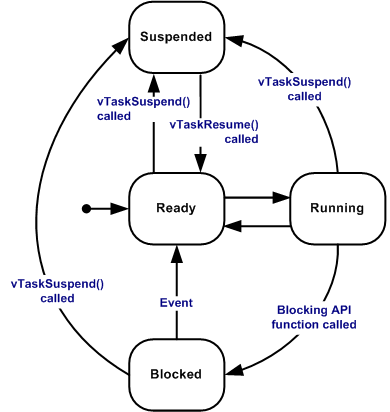
\includegraphics[width=0.6\linewidth]{./figures/tskstate.png}
 \caption{FreeRTOS task state diagram. TODO: list resource}
 \label{fig:task_states}
\end{figure}


\begin{itemize}
    \item Running: When a task is actually utilizing the processor it is said to be in the running state.
    \item Ready: A task is said to be ready if it is not utilizing the core at the moment (it is not in the running state) but is ready to run as soon as the OS decides to switch it in.
    \item Blocked: A process is blocked if it currently waiting for a temporal (e.g.: a timed delay) or an external event (e.g.: release of a shared resource).
    \item Suspended: A task is suspended if it has been told so through an explicit function call to \verb+vTaskSuspend()+.
\end{itemize}

The whole state diagram is depicted in figure~\ref{fig:task_states}. When a task gets switched in the scheduling algorithm has to decided which new task is given processor time. There are different approaches to that. For example a round robin scheduler assigns fixed time slots to every process and the different tasks are therefore provided with equal computation time. FreeRTOS pursues a slightly different approach. At the creation of each task the programmer can assign a priority to the task he is creating. Based on the priority freeRTOS schedules the next task accordingly, beginning with the highest priority task either in the ready or running state. Least precedence is given to lower priority tasks. The idle task has priority zero. If two tasks share the same priority freeRTOS schedules them in a round robin fashion.

\begin{figure}[htbp]
 \centering
 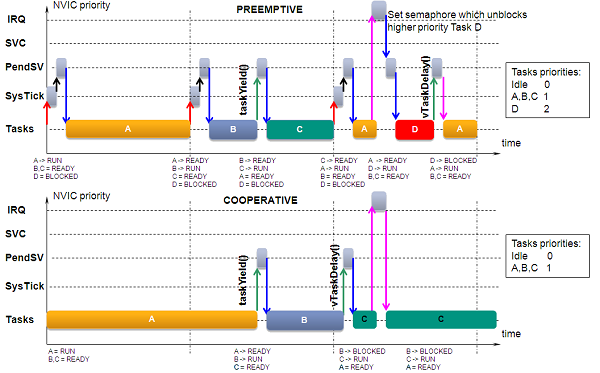
\includegraphics[width=\linewidth]{./figures/preemptive_cooperative.png}
 %https://www.rapitasystems.com/blog/cooperative-and-preemptive-scheduling-algorithms
 \caption{Preemptive and cooperative context switch}
 \label{fig:context_switch}
\end{figure}


In the preemptive case the OS needs a way to preempt a currently running task. It does this by registering a interrupt service routine (ISR) triggered by a timer that is configured by the OS according to the users specification. The interrupt triggers an asynchronous change in the control flow and directs control back to the OS that then decides whether the current task shall be switch out or not. Figure~\ref{fig:context_switch} depicted the difference between a preemptive and cooperative context switch.

\subsection{Directory structure}

Since freeRTOS aims high portability, the directory structure directly reflects this property. Everything that is architectural specific resides in the \verb+portable+ folder. This begins with basic configuration macros and continues with implementation of the actual context switch in \verb+port.c+.

\begin{minipage}{\linewidth}
\begin{flushleft}
\dirtree{%
.1 /.
  .2 main.c \DTcomment{Entry point of user program}.
  .2 FreeRTOSConfig.h \DTcomment{User defined and application specific freeRTOS configuration}.
  .2 update-ips.py \DTcomment{This script reads the ip\_list.txt and pulls all ips from the GIT server}.
  .2 include \DTcomment{Folder containing scripts used by continuous integration}.
  .2 portable \DTcomment{Contains the actual source files of your report.}.
    .3 GCC \DTcomment{Portable layer specific to GCC}.
        .3 RI5CY \DTcomment{Portable layer specific to the microcontroller's architecture}.
            .4 portmacro.h \DTcomment{architecture related configuration file}.
            .4 port.c \DTcomment{Actual portable layer implementation}.
    .3 MemMang \DTcomment{Memory management schemes.}.
  .2 event\_groups.c \DTcomment{freeRTOS eventing scheme.}.
  .2 list.c \DTcomment{List implementation - Task utility}.
  .2 tasks.c \DTcomment{Task implementation.}.
  .2 timers.c \DTcomment{Software timers.}.
}
\end{flushleft}
\end{minipage}
\subsection{Portable layer}

The portable layers purpose is to abstract all device specific information to the OS. In particular this means implementation of the actual context switch, interrupt service routines (ISRs) that trigger the context switch and stack initialization for task creation. All device specific codes resides here.

\subsection{Context Switch}

\begin{figure}[t]
 \centering
 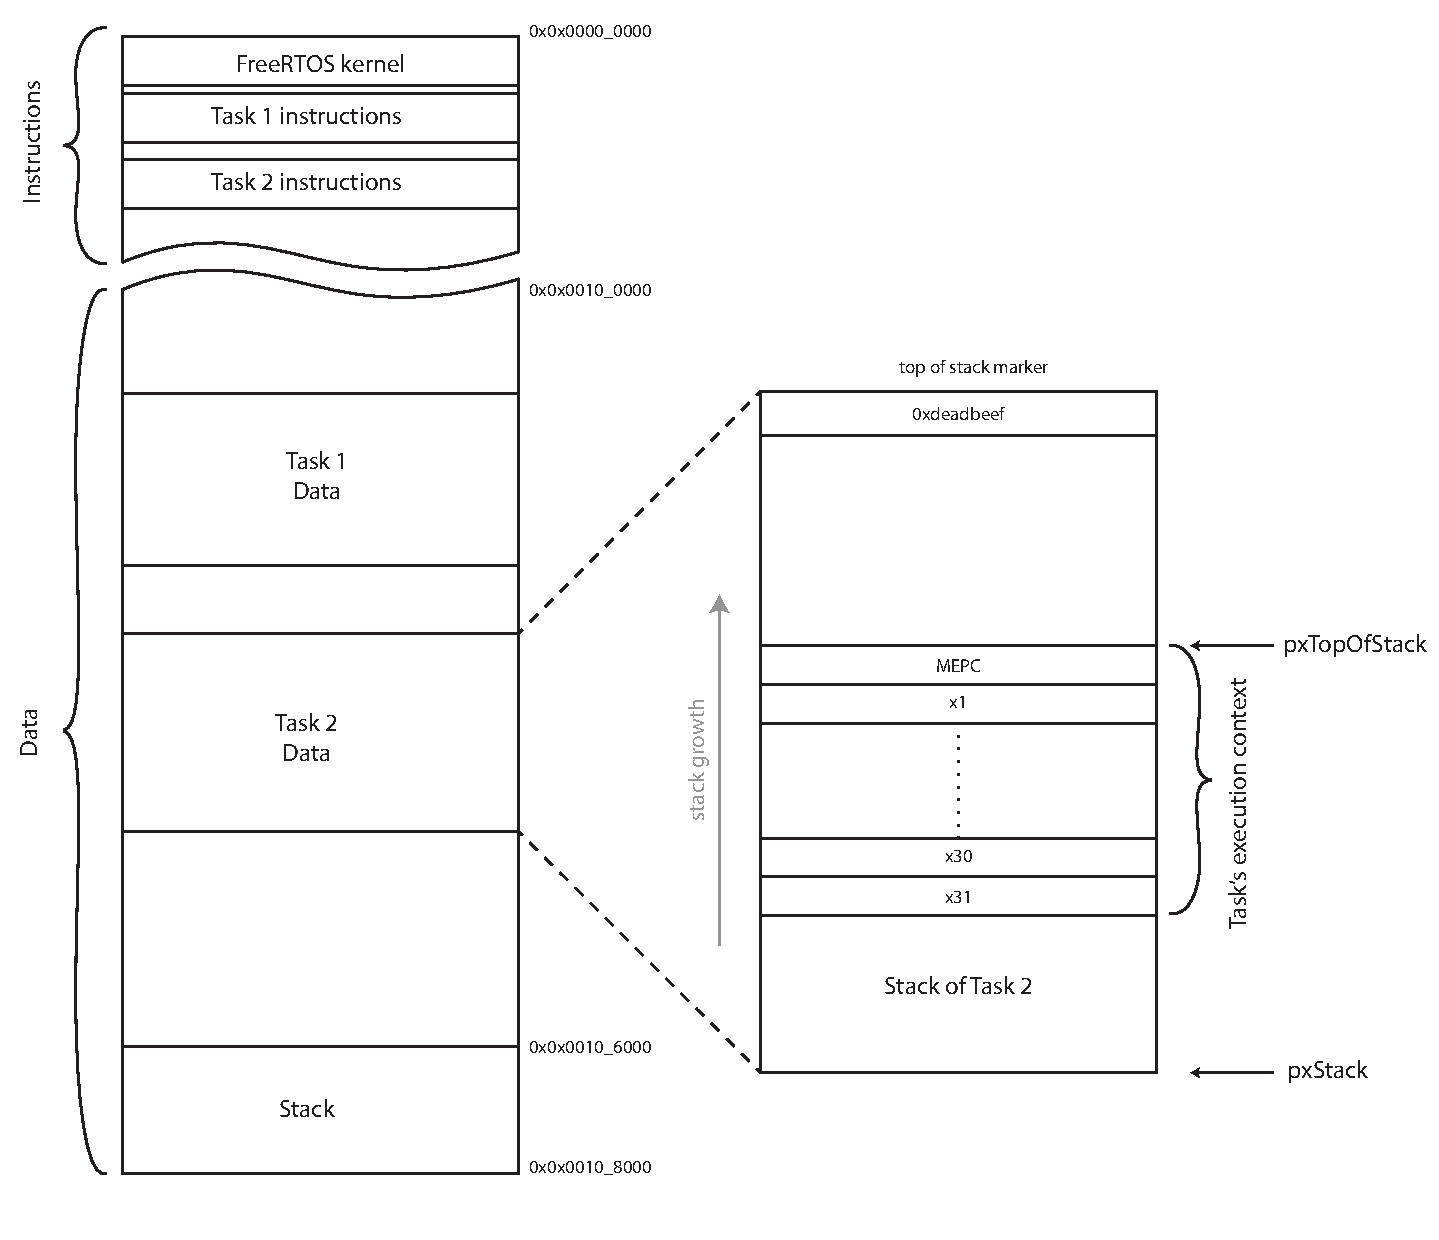
\includegraphics[width=\linewidth]{./figures/freertos_memorymap}
 %https://www.rapitasystems.com/blog/cooperative-and-preemptive-scheduling-algorithms
 \caption{FreeRTOS memory management and stack content of a switched out task (Task 2)}
 \label{fig:memory_management}
\end{figure}

Context switches can occur in two different settings depending on the scheduling algorithm in use. According to that, there are differences in the program control flow. Nevertheless the main idea of the context switch stays the same.

Each task in freeRTOS manages its own stack (figure~\ref{fig:memory_management}). The task's memory region is allocated when the tasks gets registered for the first time and reside entirely in the heap regardless of the global linker settings. In order for FreeRTOS to manage the task's memories it stores task related information in its own task structure called Task Control Block (TCB). The TCB has essentially the following structure:

\begin{figure}[t]
 \centering
 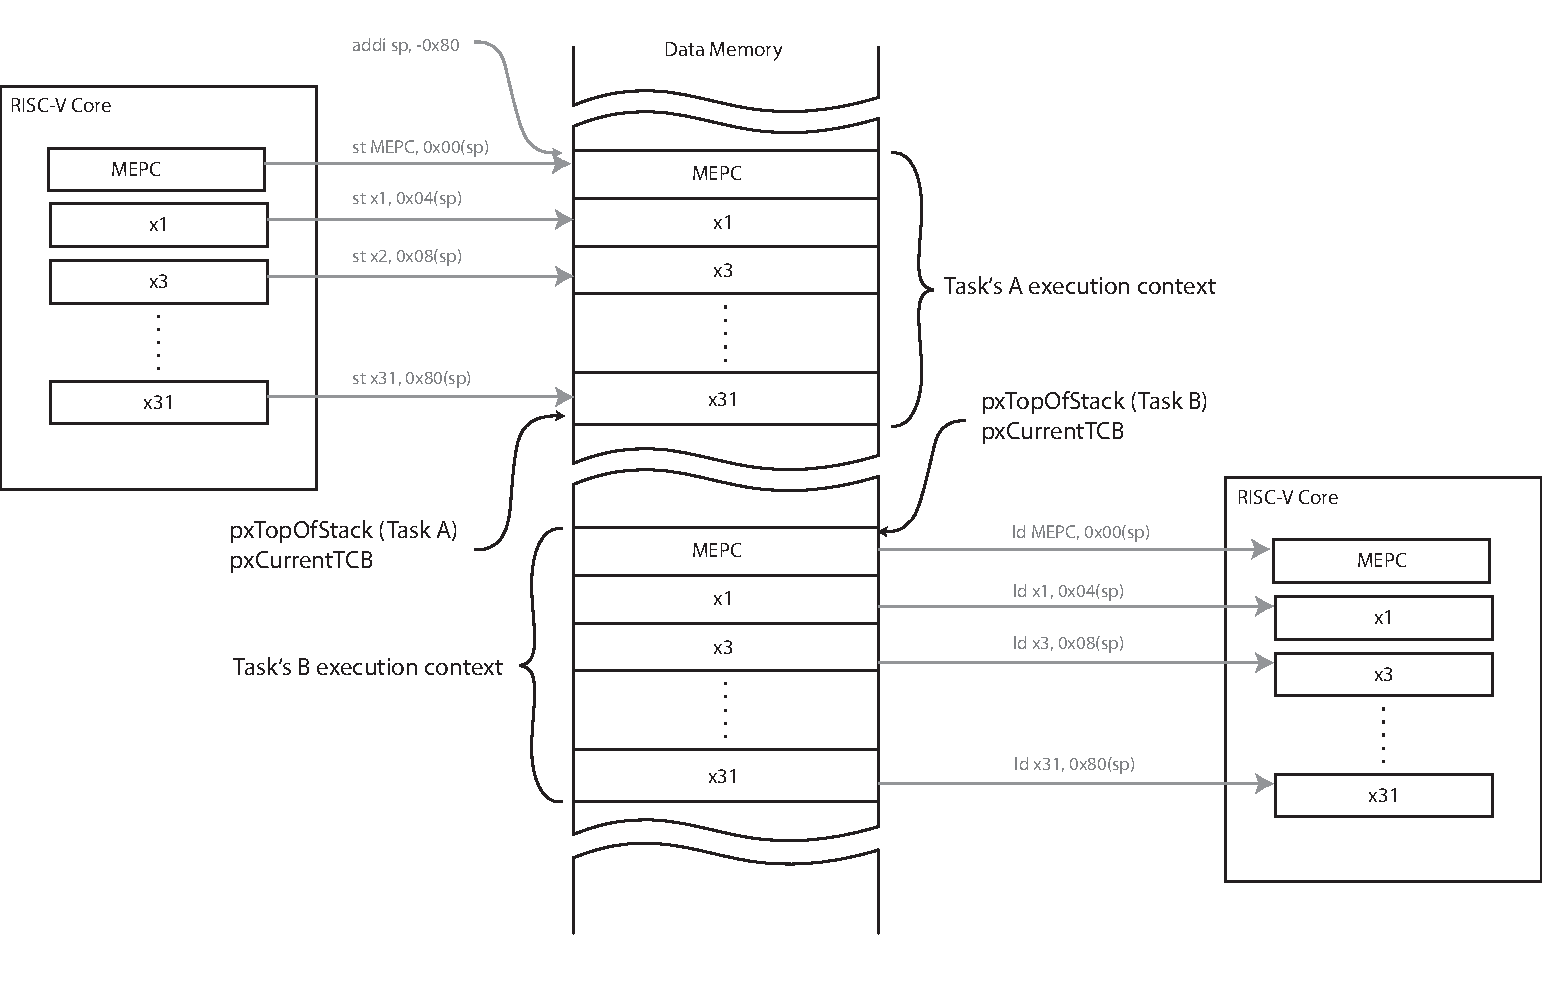
\includegraphics[width=\linewidth]{./figures/freertos_context_switch}
 %https://www.rapitasystems.com/blog/cooperative-and-preemptive-scheduling-algorithms
 \caption{FreeRTOS context switch}
 \label{fig:context_switch}
\end{figure}

%memory layout
\begin{minipage}{\linewidth}
\begin{lstlisting}[language=C,emph={xListItem,portSTACK_TYPE}]
typedef struct tskTaskControlBlock
{
  volatile portSTACK_TYPE *pxTopOfStack;
  xListItem    xGenericListItem;
  xListItem    xEventListItem;
  unsigned portBASE_TYPE uxPriority;
  portSTACK_TYPE *pxStack;
  ...
} tskTCB;
\end{lstlisting}
\end{minipage}


The \verb+pxTopOfStack+ variable points to the last element put on the stack of the task and must be the first element of the TCB structure. \verb+pxStack+ on the contrary points to the stack's base address.

If a task is switched out its current state is going to be saved into memory. For the RISC-V RV32I this implies at least all general purpose registers and the MEPC register that has the program counter stored from which the interrupt service unit may return to. It does so by calling the \verb+portSAVE_CONTEXT()+ macro defined in \verb+port.c+. This macro allocates some space on the stack and stores every register in a predefined order, starting with the MEPC. Finally it updates the \verb+pxCurrenTCB+ pointer that points to the TCB of the task switch out and updates the stack pointer. The stack pointer is therefore saved implicitly in the TCB.

The OS then figures out which task that is going to run next (based on the principles mentioned beforehand) and afterwards calls the \verb+portRESTORE_CONTEXT()+ macro. This essentially performs the same function as the save routine but in reverse order, e.g. it loads the stack pointer of the task that is going to be switched in from the pxCurrentTCB and restores all registers from memory in the same order as they have been saved.

% picture

For the cooperative case this happens within a normal function call, e.g.: a task decides that it may wants to yield and therefore gives a call to \verb+vPortYield()+. The scheduler saves the current context and restores it after it has figured out which task is going to be switched in. It is crucial that the save and restore sequence does not get interrupted therefore interrupts are disabled throughout the whole process.

For the preemptive case this happens within an ISR. The only difference to the cooperative case is that the return from the interrupt (ERET) will use the MEPC register to find out where the current task has been interrupted from.

\subsection{Stack initialization}

The purpose of the stack initialization is to setup a task structure in the data RAM to look like it has been already running and was only switched out by the scheduler. To this point the OS has already allocated some space on the stack. What remains for the initialization to do is to store the start address of the task on the same place we would have stored the return address (register x1) and the MEPC if the task has been switched out. It therefore can simply restore the context of the task albeit it has never been running before.

Remaining functionality that is architecture depended is the configuration of the timer interrupt and a call to return to directly jump to the tasks code. We have to manually call the \verb+ret+ directive since we do not want to return to the function that has called \verb+xPortStartScheduler+ but to the program.


\section{Second Section}



\part{Imperio}
%!TEX root = ../report.tex
%%%%%%%%%%%%%%%%%%%%%%%%%%%%%%%%%%%%%%%%%%%%%%%%%%%%%%%%%%%%%%%%%%%%%%%
%%%%%%%%%%%%%%%%%%%%%%%%%%%%%%%%%%%%%%%%%%%%%%%%%%%%%%%%%%%%%%%%%%%%%%%
%%%%%                                                                 %
%%%%%     architecture.tex                                            %
%%%%%                                                                 %
%%%%% Author:      Florian Zaruba                                     %
%%%%% Created:     <date>                                             %
%%%%% Description: <description>                                      %
%%%%%                                                                 %
%%%%%%%%%%%%%%%%%%%%%%%%%%%%%%%%%%%%%%%%%%%%%%%%%%%%%%%%%%%%%%%%%%%%%%%
%%%%%%%%%%%%%%%%%%%%%%%%%%%%%%%%%%%%%%%%%%%%%%%%%%%%%%%%%%%%%%%%%%%%%%%

\chapter{Hardware Architecture}

In this chapter I will give an architectural overview of the \pulpino SoC. As described in the instructional chapter both cores available for \pulpino feature a 32-bit 4-stage in order pipeline with distinct ports to the instruction and data RAMs. Since the cores are totally pin compatible one can swap them as needed without modifying any RTL.

\pulpino uses a 32-bit wide AXI as its main interconnect. The memories and the core itself are connected to the AXI Bus via dedicated bus adapters. The APB peripherals are connected to the AXI bus through a AXI2APB adapter. As all components withing the system have access to the AXI bus they share a common memory map. This makes it particularly easy to write and read registers from each peripheral, the core and memories' content. The overall device architecture is depicted in figure~\ref{fig:block_diagram}.


\begin{figure}[th]
  \centering
  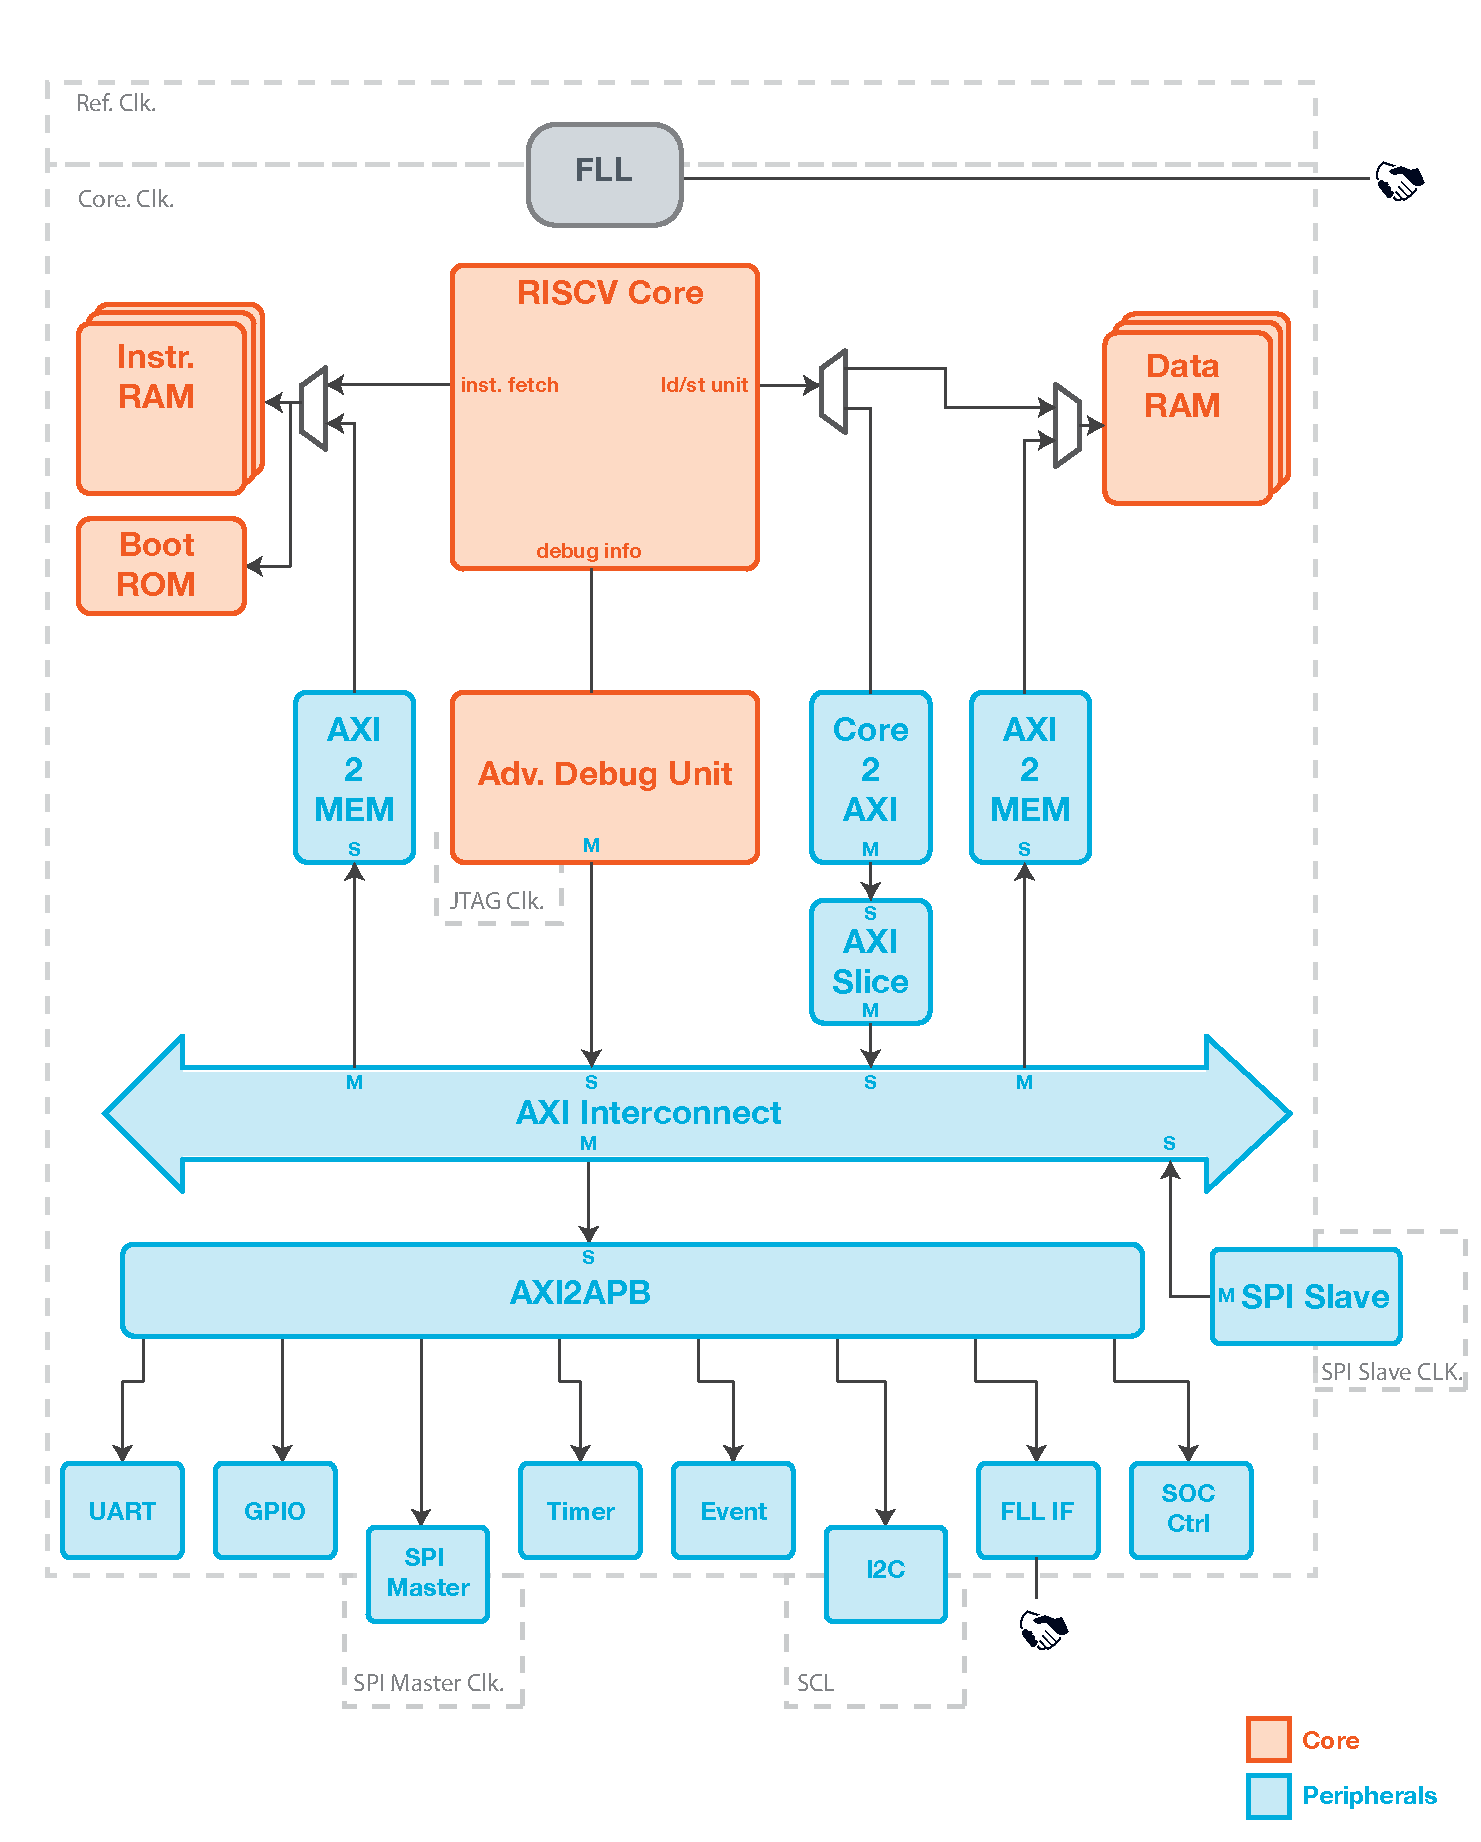
\includegraphics[width=\linewidth]{./figures/pulpino_blockdiagram}
  \caption{\pulpino block diagram}
  \label{fig:block_diagram}
\end{figure}


\section{Core}

\pulpino comes with two cores available. Both cores have been developed by the PULP group. This can either be the RISC-V core RI5CY or the pin compatible OpenRISC core OR10N.

\subsection{OpenRISC - OR10N}

OR10N was developed as part of a semester thesis here at IIS by Renzo Andri and Matthias Baer in 2014. It was meant to replace the former OpenRISC 1200 core used for the PULP project. The core employs a 32-bit 4 Stage in-order pipeline and has shown to be significantly faster then the reference implementation of the OpenCores community called OpenRISC 1200 \cite{renzobaer}.

\subsection{RISC-V - RI5CY}

RI5CY is a 4-stage in-order CPU based on the freely available RISC-V instruction set developed at UCB. The core has been mainly developed by Sven Stucki as part of his master's thesis (TODO: Citiation??). RI5CY is loosely based on OR10N. 

The RISC-V instruction set comes in a very modular and extendable flavor \cite{Waterman:EECS-2014-54}:

\begin{itemize}
    \item \textbf{RV32I}, \textbf{RV64I}: Is the 32-bit or 64-bit respectively, base integer instruction set. It describes general instruction formats and includes all operations to modify (integer) data and control flow. We fully support the bas integer instruction set with our RI5CY core.
    \item \textbf{M Standard Extension}: The M standard extension describes multiplication and division operations that multiply or divide values held in two integer registers. We provide only partial support for the M extension since our current multiplier implementation uses a single-cycle 32 bit lower result multiplier. As a matter of fact we do not support divisions and multiplications that return the upper half of the result.
    \item \textbf{A} (Atomic), \textbf{F} (single precision floating point) and \textbf{D} (double precision floating point) \textbf{standard extension}: We currently do not support any of these extensions.
    \item \textbf{C standard compressed ISA}: The compressed ISA specification is currently a proposal but will likely be frozen in the near future. The compressed ISA aims to reduce static and dynamic code size by adopting a simple compression scheme (i.e. small immediate values, one of the registers is the zero register $x0$,...). According to the current compressed ISA draft specification typically 50\%-60\% of the RISC-V instructions in a program can be replaced with RVC instructions, resulting in a 25\%-30\% code-size reduction~\cite{Waterman:EECS-2015-209}.
\end{itemize}

In addition the RISC-V ISA provides the opportunity to define instruction set extensions that are not currently officially supported. We do make particular use of this with support of post-increment load and store instructions, hardware loops and packed-SIMD instructions.


\section{AXI Interconnect}

\pulpino features an AXI bus as its main interconnect. Memories and the core are connected via dedicated bus adapters developed by the PULP group. The main advantage of having everything sharing one interconnect is the fact that the whole architecture becomes memory mapped. Resulting in the fact that 

% Axi slices

\subsection{SPI Slave}


\section{Advanced Debug Unit}

\section{APB Peripherals}

\subsection{Interrupt and Sleep Unit}

The unit is conducted as an APB peripheral. Each interrupt can be enabled or disabled and can have its pending status set or cleared by software (resulting in the fact that we support "soft interrupts"). The units main purpose is to keep track of all arriving interrupts and outputting the interrupt with the highest priority (starting from 0 up to 31) - iff it is enabled -  to the core in a one-hot encoded fashion. 

The interrupt unit can basically handle two types of interrupt sources:

\begin{itemize}
    \item \textbf{Pulsed interrupt request} - the interrupt request is at least one clock cycle long. When the interrupt controller receives a pulse at its interrupt input, the pending status is set and held until the interrupt gets served.
    \item L\textbf{evel triggered interrupt request} - the interrupt source holds the request high until the interrupt is serviced.
\end{itemize}

The interrupt output to the core is level sensitive. As long as there is a pending interrupt the corresponding interrupt request line (\verb+irq_o+) gets asserted. If the core wants to acknowledge an external interrupt it needs to clear the corresponding pending interrupt by writing 1 to the \verb+clear_pending+ (ICP) register. The interrupt is then de-asserted.

The event unit has exactly the same RTL layout as the interrupt unit. The only difference is that its \verb+signal_o+ is not forwarded to the processor core. An event can wake the core from sleep state. (TODO: provide a facility to get the currently pending event).

The sleep unit's task is to put the core into a low power mode by disabling its clock (through a clock gate). It therefore needs to track the sleep status of the core through a simple FSM (see figure~\ref{fig3}). The sleep unit is tightly coupled to the interrupt unit since it needs to wake the processor if an enabled interrupt arrives.
The sleep controller is as well conducted as an APB peripheral with two registers (see figure~\ref{fig4}):

\begin{enumerate}
    \item \textbf{Sleep Controll Register:} By writing the lowest bit (SE - Sleep Enable) to 1 the core requests to be put to sleep. Upon wakeup this bit is cleared by the controller.
    \item \textbf{Sleep Status Register:} This register contains the current sleep status of the core. This is helpful if for example you want to get the sleep status through the debug interface. Writes to this location are ignored.
\end{enumerate}

If the core signals that it is idle and wants to be put to sleep it writes the SE register. The controller then enters the \verb+SHUTDOWN+ state where the fetch enable signal of the core is de-asserted and no more instructions are fetched. After the processor has flushed its pipeline (signaled by a low \verb+core_busy+ signal) its clock is gated and the \verb+SLEEP+ state is entered. It now resides in a lower power state and can only be waked up by an external interrupt event (\verb+signal_i+ asserted).

\subsection{Timer Unit}

The timer provides a facility to cycle accurately time certain events and/or trigger interrupts or events respectively. In detail it should be possible to generate a timer overflow interrupt/event if the timer reaches its highest value and a timer output compare event when the timer is equal to a certain value set in the timer output compare register.


Additionally a timer control register makes it possible to set a pre-scaler, enable/disable timer overflow and timer output compare interrupts/events and to start and stop the timer respectively.

\subsection{\pulpino peripheral}

In order to control certain features of the SoC a special set of control registers is needed to do so. Since this is highly application specific (e.g. it only applies to this distinct SoC configuration) it has been my indention to logically and physically separate this sort of functionality into an independent peripheral.

Specificially this peripheral allows you to control the function of pads (e.g. whether they should be used as GPIO or perform there special function like SPI, UART, etc.). Furthermore this unit allows you to reconfigure the boot address. The boot address is the address the core stars fetching instructions as soon as the fetch enable signal of the core has been asserted.

\subsection{I2C}

\subsection{UART}

\subsection{SPI Master}









%!TEX root = ../report.tex
%%%%%%%%%%%%%%%%%%%%%%%%%%%%%%%%%%%%%%%%%%%%%%%%%%%%%%%%%%%%%%%%%%%%%%%
%%%%%%%%%%%%%%%%%%%%%%%%%%%%%%%%%%%%%%%%%%%%%%%%%%%%%%%%%%%%%%%%%%%%%%%
%%%%%                                                                 %
%%%%%     06_implementation.tex                                       %
%%%%%                                                                 %
%%%%% Author:      Florian Zaruba                                     %
%%%%% Created:     13.12.2015                                         %
%%%%% Description: <description>                                      %
%%%%%                                                                 %
%%%%%%%%%%%%%%%%%%%%%%%%%%%%%%%%%%%%%%%%%%%%%%%%%%%%%%%%%%%%%%%%%%%%%%%
%%%%%%%%%%%%%%%%%%%%%%%%%%%%%%%%%%%%%%%%%%%%%%%%%%%%%%%%%%%%%%%%%%%%%%%


\chapter{Design Implementation and Results}

This chapter is about the implemented functionality and ASIC key design data (timing, area and power) and implementation decisions made.

\section{Implementation}

\subsection{Multiplexed Pads}

Since pads are often a quite limiting factor in the overall design it can be particularly useful to reuse them depending on the functionality required at a certain point in time.

The pads should remain highly configurable. Therefore it was necessary to multiplex all inputs and outputs of every pad instance that should perform a secondary function (for example function as an UART or GPIO). Depending on a configuration register in the APB \pulpino Peripheral (\ref{subsec:pulpino_peripheral}) the pad should switch functionality. In addition all pads need to be in a fixed configuration when the chip is on the tester (testmode is enabled).

The block diagram of the pad multiplexers is depicted in figure~\ref{fig:pad_muxes}. In order to not clutter the circuit diagram too much output enable, input, output and configuration multiplexers are drawn for different functionality of the circuit. In fact all pins that share functionality feature all multiplexers depicted.
\begin{itemize}
    \item \textbf{Output Enable (OE)}: For the pads primary function output is either tied to low or high depending on the main functionality. If the pad is configured as general purpose I/O it is connected to the configuration register of the APB GPIO module (see~\ref{subsec:gpio_peripheral}).
    \item \textbf{Input}: If the pad serves double functionality, in terms of that its primary function serves as input, its input pin is multiplexed to the main entity. Depending on how the pad is currently configured the the non-active input is silenced.
    \item \textbf{Output}: If the pad serves as an output in its primary function the output to the pad is selected in terms of its current configuration.
    \item \textbf{Pad Config}: Pad configuration is a 6 bit wide bus that sets the pads configuration, depending on its current functionality, accordingly (like Schmitt Trigger, Drive Strength, etc.).
\end{itemize}
An exhaustive pad list along with reset configuration values is depicted in the chip's data-sheet (\ref{tab:pads})).


\begin{figure}[tbh]
  \centering
  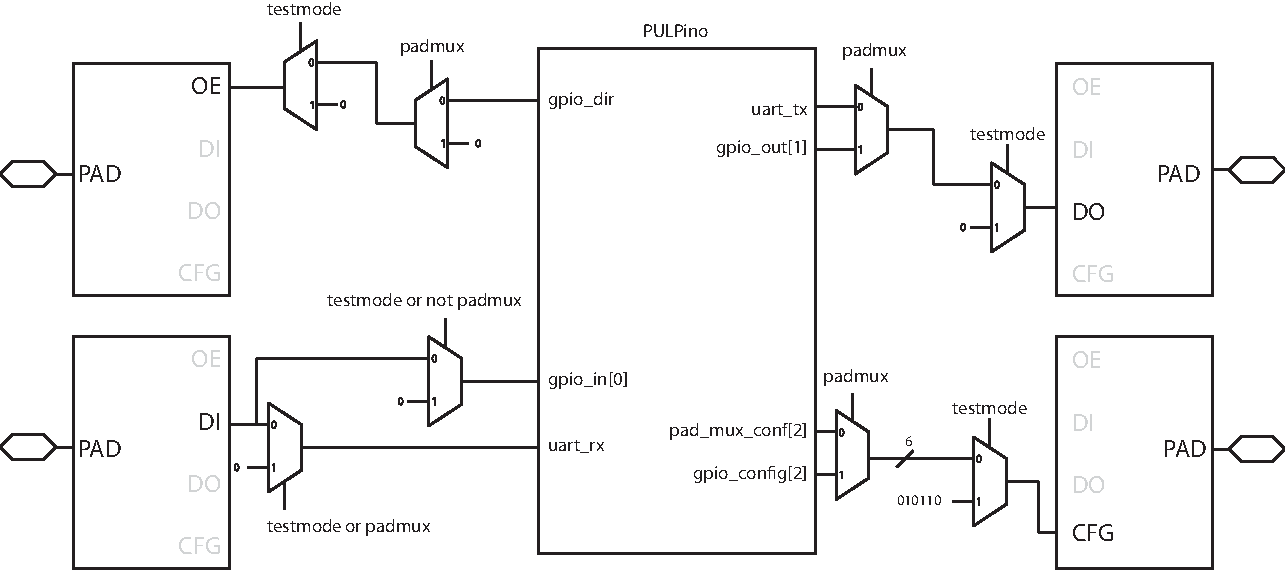
\includegraphics[width=\linewidth]{./figures/pad_muxes}
  \caption{Multiplexed Pads}
  \label{fig:pad_muxes}
\end{figure}

\subsection{Register file}
% Latch based vs. register based register file

\subsection{RAM banks}
%relate to timing

\section{Booting}

Booting is an essential part of the ASIC implementation. Unless you are really accounting for loading program data into the microcontroller you are left with a worthless piece of silicon. The boot process on Imperio is achieved by a 2 kByte of boot ROM that has instructions that read a SPI Flash and load instructions and data into memories.

The compiled program is stored in the SPI Flash. It starts at address zero with 32 bytes of meta data that tell the bootcode where the instruction section begins, how many bytes are used to encode each instruction, where it should start fetching and how may blocks of fixed length it has to expect. The same is done for the data.

A special script takes care of preparing the flash content. This means calculating the headers and formatting the instructions.

The core starts executing boot code unless otherwise explicitly told so by writing the start address registers in the \pulpino APB peripheral (see~\ref{subsec:pulpino_peripheral})). 

The boot sequence starts by reading the vendor ID of the connected SPI Flash (we are only supporting a certain type of SPI Flash, where we definitely know all timing parameters). Next the SPI Master switches the communication to Quad SPI which is an extension to standard SPI but with 4 bidirectional data lanes. This has the advantage of providing a speedup of four times.

Next, the processor reads the 32 byte of header information and starts by loading instruction data into its instruction RAM. Afterwards the same is done for the data section of the program. Finally it jumps to the base of the instruction RAM and starts executing the main program.

During the boot process interrupts are disabled and all peripherals except the SPI Master are in reset configuration. For the full boot code refer to~\ref{sec:boot_code}.

\label{sec:booting}


\section{Verification}

This section deals with functional and circuit level verification. In the functional section I will give detailed explanation on how \pulpino and Imperio are tested.

\subsection{Functional}

For functional verification we mainly distinguish two test settings: \pulpino related functional verification and imperio related verification. One can see Imperio's test setting as superset of \pulpino's e.g. every test that can be run on \pulpino can also be conducted on Imperio but not vice-verse.

\subsubsection{\pulpino testbench}

\pulpino tests are performed in a platform setting. This means that the core gets instantiated in the target platform setting and is then tested exclusively in this environment. This provides the advantage of having a very generic test framework which allows us to test (high level) assembly and C code. We have a specialized test library in place that performs checks for errors and generates reports that are output over UART. Currently we are supporting two different kind of tests:
\begin{enumerate}
    \item \textbf{Sequential Tests:} Pure C code tests that perform common micro-benchmarks like sorting, matrix multiplication.
    \item \textbf{RISC-V Tests:} Test that are exercising certain features of the core. This group also contains Berkely's official RISC-V tests that have been ported in the course of RI5CY's development. Additionally we are testing load/stores, control flow instructions and our instruction set extensions amongst others.
\end{enumerate}

The testbench is highly configurable through parameters that are set when the corresponding testbench script is invoked (see the \verb+vsim/scripts+ folder for a list of available configurations see~\ref{subsec:directory_structure}). I want to emphasize two particular configuration parameters namely clock select and memload. 

The first one selects whether the core should be clocked by an external reference clock or by its internal FLL. In terms of RTL simulation this does not matter too much since we do not have any timing parameters that may prevent us to use higher clock speeds through the external clock generation. But it allows for functional verifying the FLL.

The memload parameters specifies how the memories of the DUT should be filled with instructions and data. For \pulpino we support:
\begin{itemize}
    \item \textbf{Memory pre-loading}: In this setting we make use of the fact that we can directly pre-load the memories' functional model. Prior to starting the core all memories are filled with the content of \verb+.slm+ files that have been created of the corresponding object file with special conversion scripts (located in \verb+sw/utis/+).
    \item \textbf{SPI Slave}: As discussed in the SPI Slave Section (\ref{subsec:spi_slave}) \pulpino's entire memory region can be written from outside via SPI. This makes it possible to load instructions and data through SPI.
    \item \textbf{JTAG}: Since the whole memory region is mapped to a common address space it is possible to write the RAMs through JTAG as well. Therefore it is possible to load a program via JTAG.
\end{itemize}

After the program has been loaded by either of the three possibilties specified above the fetch enable signal gets asserted and the core start computation. Depending on the test currently running the results are checked against a golden model.  This can either be some constants that where computed prior to compilation or other entities that get checked, for example a certain register's content.

Once the test passed this check this is reported back to the test bench library that outputs a fixed string over UART. This string either gets checked manually or automatically by the \verb+run_and_check.py+ python script.

\subsubsection{Imperio testbench}

For Imperio's testbench the approach is very similar. Actually the only reason why we employ a different test bench for ASIC related tests is, on the one hand, the reason that we are not allowed to open-source the models like that of the SPI Flash or I2C EEPROM and therefore need a clean separation. On the other hand the top instances of \pulpino are different in regard of input and output. While for \pulpino there are only one-directional I/O this is not longer the case for Imperio sine we have the padframe in between.

\subsubsection{Imperio RTL Simulation}

As mentioned above Imperio's testbench extends the environment of \pulpino's testbench in terms of that it instantiates behavioral models of two I2C EEPROMs and one SPI Flash. This has two advantages:
\begin{enumerate}
    \item Using models in the testbench better simulates the PCB environment the ASIC is finally going to be employed.
    \item It allows us to use a special boot sequence to load instructions and data from an external memory. In the case of Imperio this is going to be a Spansion SPI Flash. For the detailed boot code refer to the appendix~\ref{sec:boot_code} and for an explanation of the boot process to section~\ref{sec:booting}.
\end{enumerate}


\subsubsection{Post Synthesis Simulation}
\subsubsection{Post Layout Simulation}
% post synthesis 
% post layout

% scan chains

\subsubsection{Continuous Integration}
\begin{figure}[tb]
  \centering
  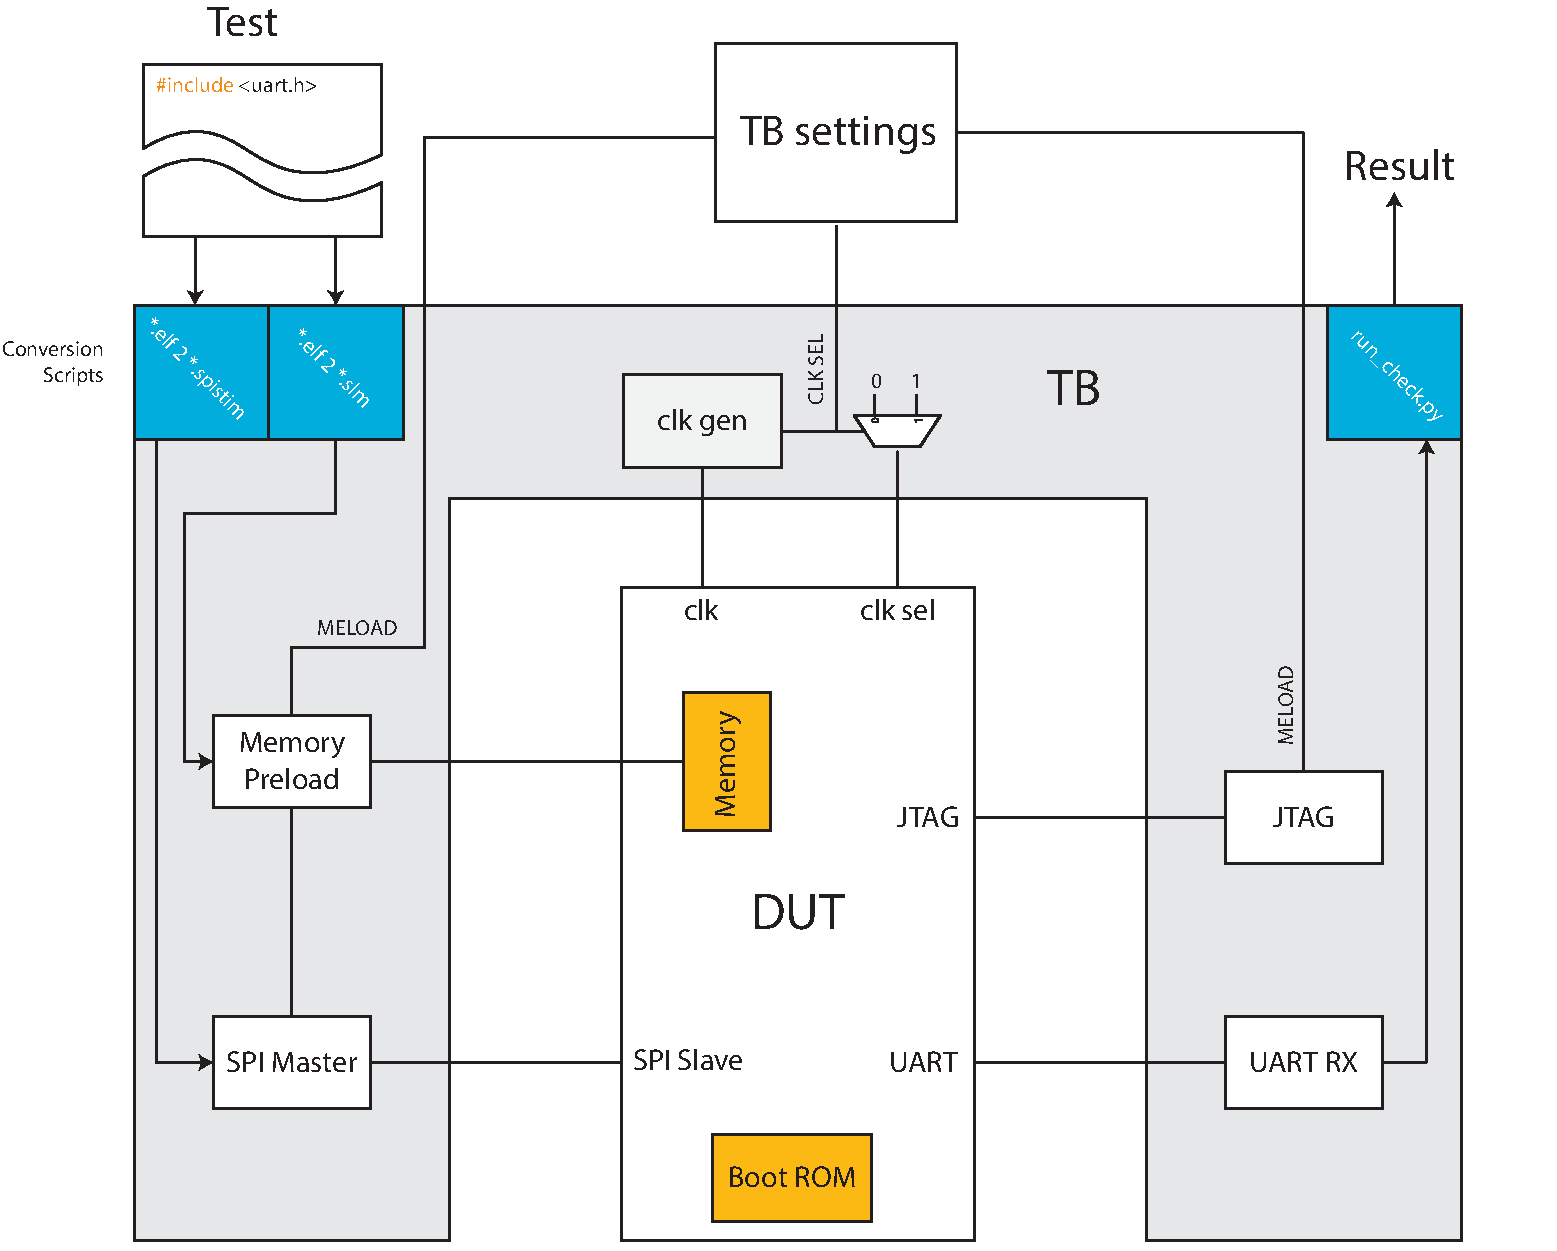
\includegraphics[width=\linewidth]{./figures/test_environment}
  \caption{Functional verification setup.}
  \label{fig:func_ver}
\end{figure}

\subsection{Design for Testability (DFT)}

The RAM's input is bypassed in test mode in order to enable scan testing the combinatorial logic around the RAM. This is especially important for the RAM2AXI interfaces which allow operations on the bare memory. Furthermore, in order to observe the address pins of the RAM observation registers for the RAM address port have been added. The area overhead is small since Synopsys uses some sophisticated techniques to, on the one hand reuse the observation registers for both the instruction and the data RAM and on the other hand, only a few registers are necessary to make the signals of interest observable. \\
The memories itself will be tested with direct access through the JTAG interface. \\
The FLL has a dedicated DFT structure featuring a ScanEnable, ScanIn and ScanOut port. Until now the FLL is not part of one of the scan chains. \\
The current DFT numbers are related to post synthesis netlists. In a first run, a couple of weeks ago, I was able to achieve a bit more than 99 \% test coverage. While in the latest runs, most probably related to the newly instantiated pad frame and the FLL, test coverage deteriorated a bit and I am at 97\% for the current design. \\


\begin{lstlisting}
     Uncollapsed Stuck Fault Summary Report
 -----------------------------------------------
 fault class                     code   #faults
 ------------------------------  ----  ---------
 Detected                         DT     351339
 Possibly detected                PT         68
 Undetectable                     UD       1267
 ATPG untestable                  AU       8065
 Not detected                     ND         99
 -----------------------------------------------
 total faults                            360838
 test coverage                            97.72%
 fault coverage                           97.38%
 -----------------------------------------------
\end{lstlisting}

\subsubsection{Automated Testpattern Generation}

\section{Area}

On the final design there is approximately 25\% core area left (on a ninth module). Detailed area results are listed in figure~\ref{fig:area}. Note that the RAMs are no longer listed as a separate design entry as they are completely ungrouped for better synthesis results. Pad instances do not show up as seperate design entries since they are not over 1 kGE alone, but accumulated they are a significant part of the overall area.

% ------- Python generated ---------
\begin{figure}[ht!]
\centering
\begin{tabularx}{\textwidth}{Xllllll}
\textbf{Entity} &  \multicolumn{3}{l}{\textbf{Total Cells (kGE)}}  &  \multicolumn{3}{l}{\textbf{\% Total}}  \\\hline
imperio&700&&&100.0&&\\
pulpino\_i&500&&&73.1&&\\
$\quad$axi\_interconnect\_i&&6&&&1.0&\\
$\quad\quad$axi\_node\_i&&&6&&&1.0\\
$\quad\quad$others &&&0&&&0\\
$\quad$clk\_rst\_gen\_i&&12&&&1.8&\\
$\quad\quad$others &&&0&&&0.0\\
$\quad$core\_region\_i&&400&&&63.6&\\
$\quad\quad$RISCV\_CORE&&&40&&&5.8\\
$\quad\quad$adv\_dbg\_if\_i&&&5&&&0.8\\
$\quad\quad$axi\_slice\_core2axi&&&2&&&0.4\\
$\quad\quad$data\_mem\_axi\_if&&&5&&&0.8\\
$\quad\quad$instr\_mem\_axi\_if&&&5&&&0.8\\
$\quad\quad$others &&&0&&&0.0\\
$\quad$peripherals\_i&&50&&&6.8&\\
$\quad\quad$apb\_event\_unit\_i&&&3&&&0.5\\
$\quad\quad$apb\_gpio\_i&&&3&&&0.5\\
$\quad\quad$apb\_i2c\_i&&&1&&&0.2\\
$\quad\quad$apb\_pulpino\_i&&&2&&&0.3\\
$\quad\quad$apb\_spi\_master\_i&&&8&&&1.2\\
$\quad\quad$apb\_timer\_i&&&3&&&0.5\\
$\quad\quad$axi2apb\_i&&&1&&&0.2\\
$\quad\quad$axi\_spi\_slave\_i&&&8&&&1.3\\
$\quad\quad$i\_apb\_uart&&&14&&&2.1\\
$\quad\quad$others &&&0&&&0.0\\
\end{tabularx}
\caption{Area estimates (UMC65 - LVT 1.2V) @ 1.3ns - 1 GE = 1.44 \textmu m$^2$}
\label{fig:area}
\end{figure}
% ------- Python generated ---------

\begin{figure}[tb]
  \centering
  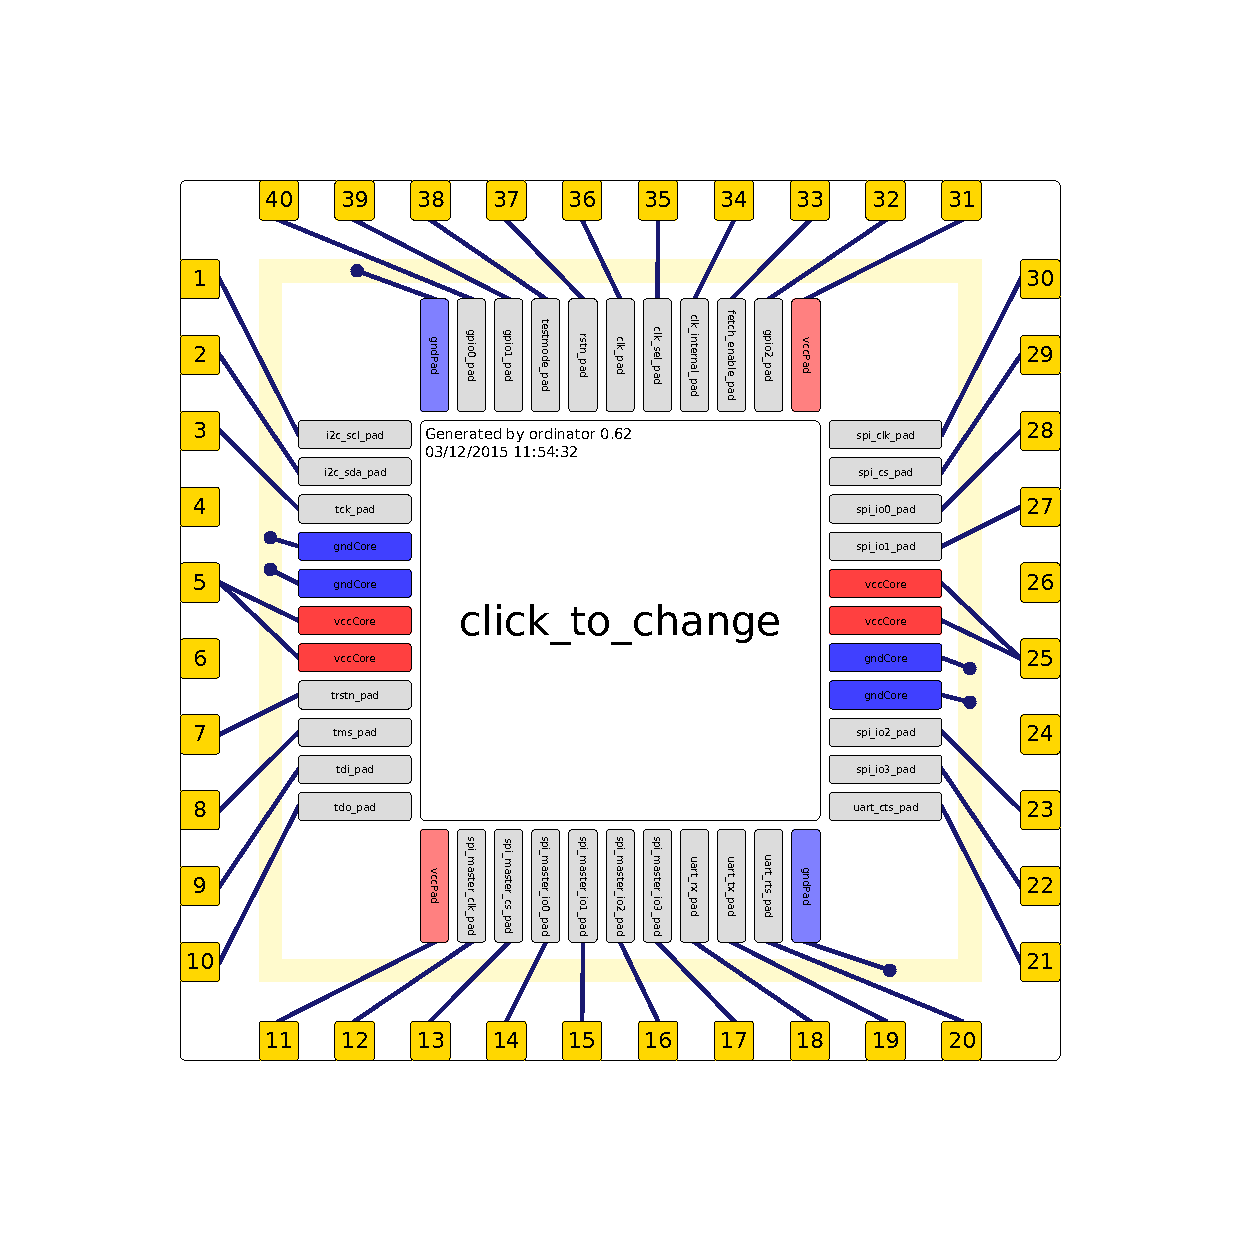
\includegraphics[width=\linewidth]{./figures/pad_instaces_img_ord}
  \caption{Bonding diagram}
  \label{fig:bonding_diagram}
\end{figure}

\section{Timing}

%talk about timing and how timing closure was achieved. useful skew, skew general relate to RAM bank implementation

\section{Power}

% power analysis

Lowering power has always been a key driving factor for the PULP group. As a matter of fact power consumption has been a point of interest for \pulpino as well. Nevertheless due to \pulpino's simplicity we spare most of the power saving tricks used by PULP. 

In order to estimate power consumption I extended the current testbench to automatically trigger ModelSim's VCD dumps. Additionally I configured the CMake environment (for more information you may want to check the Getting Started Guide~\ref{sec:getting_started}) to have a distinct power target. This makes it particularly easy to run a power estimation.

For the time being I conducted three different measurements that are mostly representative for Imperio's application context.

\begin{enumerate}
    \item Interrupt Test: The core is clock gated most of the time in this scenario. It is woken up periodically and performs an UART transaction when it wakes up.
    \item Hello World: Trivial UART output. The core is not put to a particular low power state. Most of the operations are memory operations (instruction and data fetches).
    \item Matrix Multiplication: Computational intensive operation. The core needs to fetch a lot of data from the memories and performing computational costly operations, like multiplications and additions on it. This case should be representative for high density computation. 
\end{enumerate}

Power consumption can be split up into the following three components~\cite{Kaeslin08}:
\begin{itemize}
    \item Internal power $P_{int}$: power dissipated for charging and discharging the cell's internal capacitances.
    \item Switching power $P_{ext}$: this amounts to the power that gets dissipated for charging external load capacitances (input capacitance of driven cell plus wire capacitances) that are connected to the cell's output(s).
    \item Leakage power $P_{leak}$: power dissipated by the cell in absence of switching activity.
\end{itemize}
The total power dissipated by the circuit is the sum of these:
\[
    P_{tot} = P_{int} + P_{ext} + P_{leak}
\]
All power simulations where performed at 500 MHz, 1.2 V and 25 \textdegree C. Detailed results are depicted in table~\ref{tab:power}.

\begin{table}[htbp]
 \caption{Power Results (UMC65 - LVT 1.2V) @ 2ns, 25 \textdegree C}
 \label{tab:power}
\begin{tabularx}{\textwidth}{|X||l|l||l|l||l|l||l|}
  \hline
  \textbf{Test} & $P_{int}$& \% & $P_{ext}$ &  \% & $P_{leak}$ &  \% & $P_{tot}$\\ \hline
Interrupt Test & 7.10 & 57.84 & 5.00 &  40.64 & 0.17 & 1.52 & 12.28 \\ \hline
Hello World & 19.80 & 59.64 & 13.25 & 39.88 & 0.19 & 0.56 & 33.23 \\ \hline
Mat. Mul. & 32.00 & 60.00 & 21.17 & 39.68 & 0.19 & 0.35 & 53.35 \\ \hline
  \end{tabularx}
  \end{table}


% \section{Results}


% If you only have very few results, it might be a better approach to
% insert them into this chapter (instead of putting the results into a
% separate one).



%%%%%%%%%%%%%%%%%%%%%%%%%%%%%%%%%%%%%%%%%%%%%%%%%%%%%%%%%%%%%%%%%%%%%%%
%%%%%%%%%%%%%%%%%%%%%%%%%%%%%%%%%%%%%%%%%%%%%%%%%%%%%%%%%%%%%%%%%%%%%%%
%%%%%                                                                 %
%%%%%     <file_name>.tex                                             %
%%%%%                                                                 %
%%%%% Author:      <author>                                           %
%%%%% Created:     <date>                                             %
%%%%% Description: <description>                                      %
%%%%%                                                                 %
%%%%%%%%%%%%%%%%%%%%%%%%%%%%%%%%%%%%%%%%%%%%%%%%%%%%%%%%%%%%%%%%%%%%%%%
%%%%%%%%%%%%%%%%%%%%%%%%%%%%%%%%%%%%%%%%%%%%%%%%%%%%%%%%%%%%%%%%%%%%%%%

\chapter{Results}
If you have a large amount of results you can move them to this
separate chapter.

\section{First Section}


\section{Second Section}




%!TEX root = ../report.tex
%%%%%%%%%%%%%%%%%%%%%%%%%%%%%%%%%%%%%%%%%%%%%%%%%%%%%%%%%%%%%%%%%%%%%%%
%%%%%%%%%%%%%%%%%%%%%%%%%%%%%%%%%%%%%%%%%%%%%%%%%%%%%%%%%%%%%%%%%%%%%%%
%%%%%                                                                 %
%%%%%     <file_name>.tex                                             %
%%%%%                                                                 %
%%%%% Author:      <author>                                           %
%%%%% Created:     <date>                                             %
%%%%% Description: <description>                                      %
%%%%%                                                                 %
%%%%%%%%%%%%%%%%%%%%%%%%%%%%%%%%%%%%%%%%%%%%%%%%%%%%%%%%%%%%%%%%%%%%%%%
%%%%%%%%%%%%%%%%%%%%%%%%%%%%%%%%%%%%%%%%%%%%%%%%%%%%%%%%%%%%%%%%%%%%%%%

\chapter{Conclusion and Future Work}
% Draw your conclusions from the results you achieved and summarize your
% contributions. Comparisons (e.g., of hardware figures) with related
% work are also appropriate here. Point out things that could or need to
% be investigated further.

\section{Conclusion}

My contributions to the project have been very divers. This begins with the implementation of freeRTOS on the software side as well as on the hardware side with the implementation of the timer and interrupt peripherals. Those peripherals are simpler than the ones used by PULP and therefore better fitting our needs.

Moreover I contributed to the build and verification framework of PULP/\pulpino by implementing new features like for example the core trace annotation as well as improving already implemented features like rewriting the the testbench's JTAG and SPI interfaces in a more object oriented fashion.

Finally I designed a well performing ASIC in terms of high speed and low power requirements.

\section{Future Work}

Imperio will be taped out in the end of January 2015. Since it has always been designed to be employed on a PCB this will certainly be some work that needs to be done. In particular it would be nice to have an development board that makes use of all of Imperio's features and peripherals. Furthermore it will be necessary to develop software in order to program Imperio accordingly.

Another aspect that should not be lost sight of is the support for the open source community. It will be crucial for the widespread gain of \pulpino to have a community that is using and supporting it for their own projects and products. Especially at the beginning support will be one of the key driving factors for successful project.

Lastly I am hoping that the design is going to be employed in an educational aspect and that everybody has the possibility to learn as much as I did during this semester theses.


%%%%%
%%%%% Start of additional parts.
%%%%%
\appendix

%%%%%%%%%%%%%%%%%%%%%%%%%%%%%%%%%%%%%%%%%%%%%%%%%%%%%%%%%%%%%%%%%%%%%%%
%%%%%%%%%%%%%%%%%%%%%%%%%%%%%%%%%%%%%%%%%%%%%%%%%%%%%%%%%%%%%%%%%%%%%%%
%%%%%                                                                 %
%%%%%     <file_name>.tex                                             %
%%%%%                                                                 %
%%%%% Author:      <author>                                           %
%%%%% Created:     <date>                                             %
%%%%% Description: <description>                                      %
%%%%%                                                                 %
%%%%%%%%%%%%%%%%%%%%%%%%%%%%%%%%%%%%%%%%%%%%%%%%%%%%%%%%%%%%%%%%%%%%%%%
%%%%%%%%%%%%%%%%%%%%%%%%%%%%%%%%%%%%%%%%%%%%%%%%%%%%%%%%%%%%%%%%%%%%%%%

\chapter{Task Description}
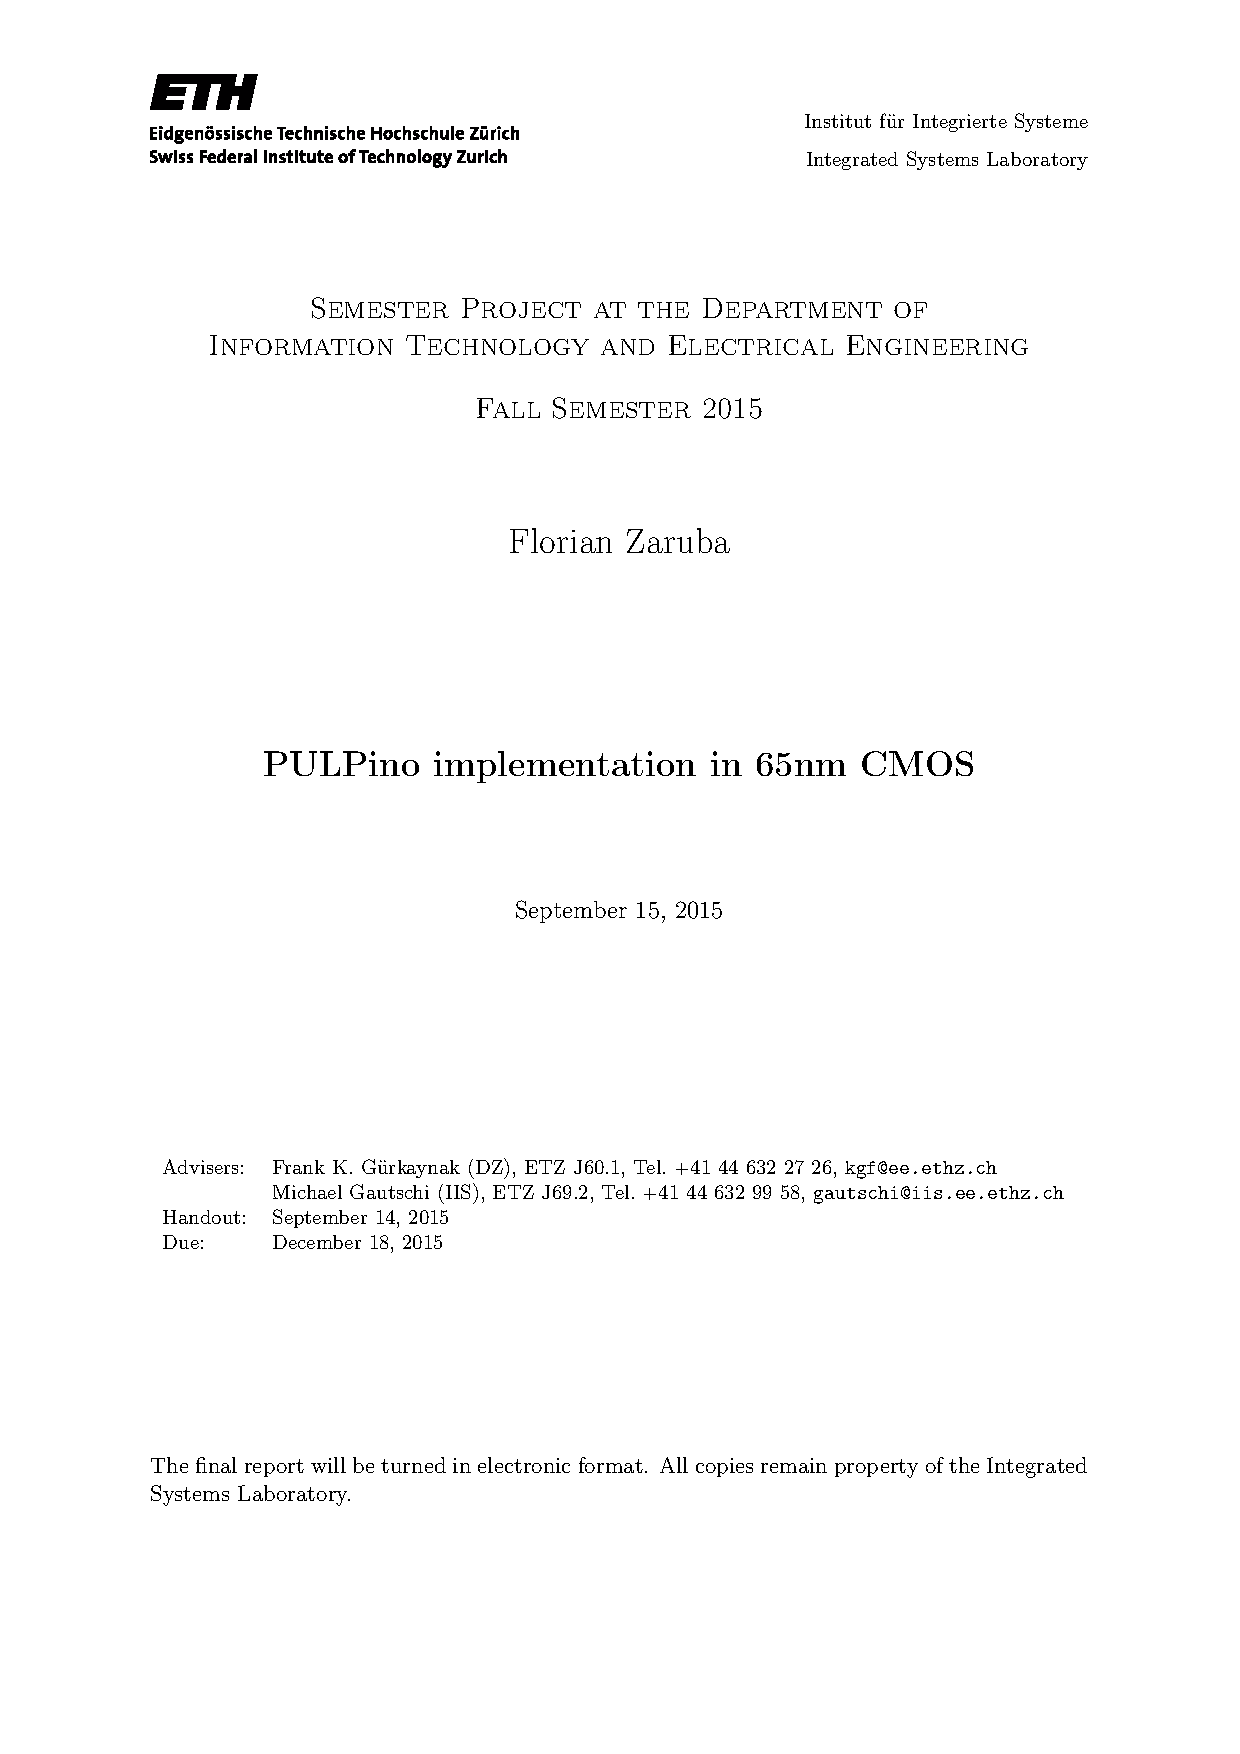
\includepdf[pages=-, turn=false, scale=0.9]{task/TaskDescription.pdf}


\chapter{Declaration of Originality}\label{chap:originality}
Include the declaration of authorship with the \shell{\textbackslash
  includepdf} command (sign it and scan it). For more information
about plagiarism, please visit
\url{https://www.ethz.ch/students/en/studies/performance-assessments/plagiarism.html}

\begin{itemize}
\item \textbf{English version:}
  \url{https://www.ethz.ch/content/dam/ethz/main/education/rechtliches-abschluesse/leistungskontrollen/declaration-originality.pdf}
\item \textbf{German version:}
  \url{https://www.ethz.ch/content/dam/ethz/main/education/rechtliches-abschluesse/leistungskontrollen/plagiat-eigenstaendigkeitserklaerung.pdf}
\end{itemize}

% include the signed declaration of authorship!
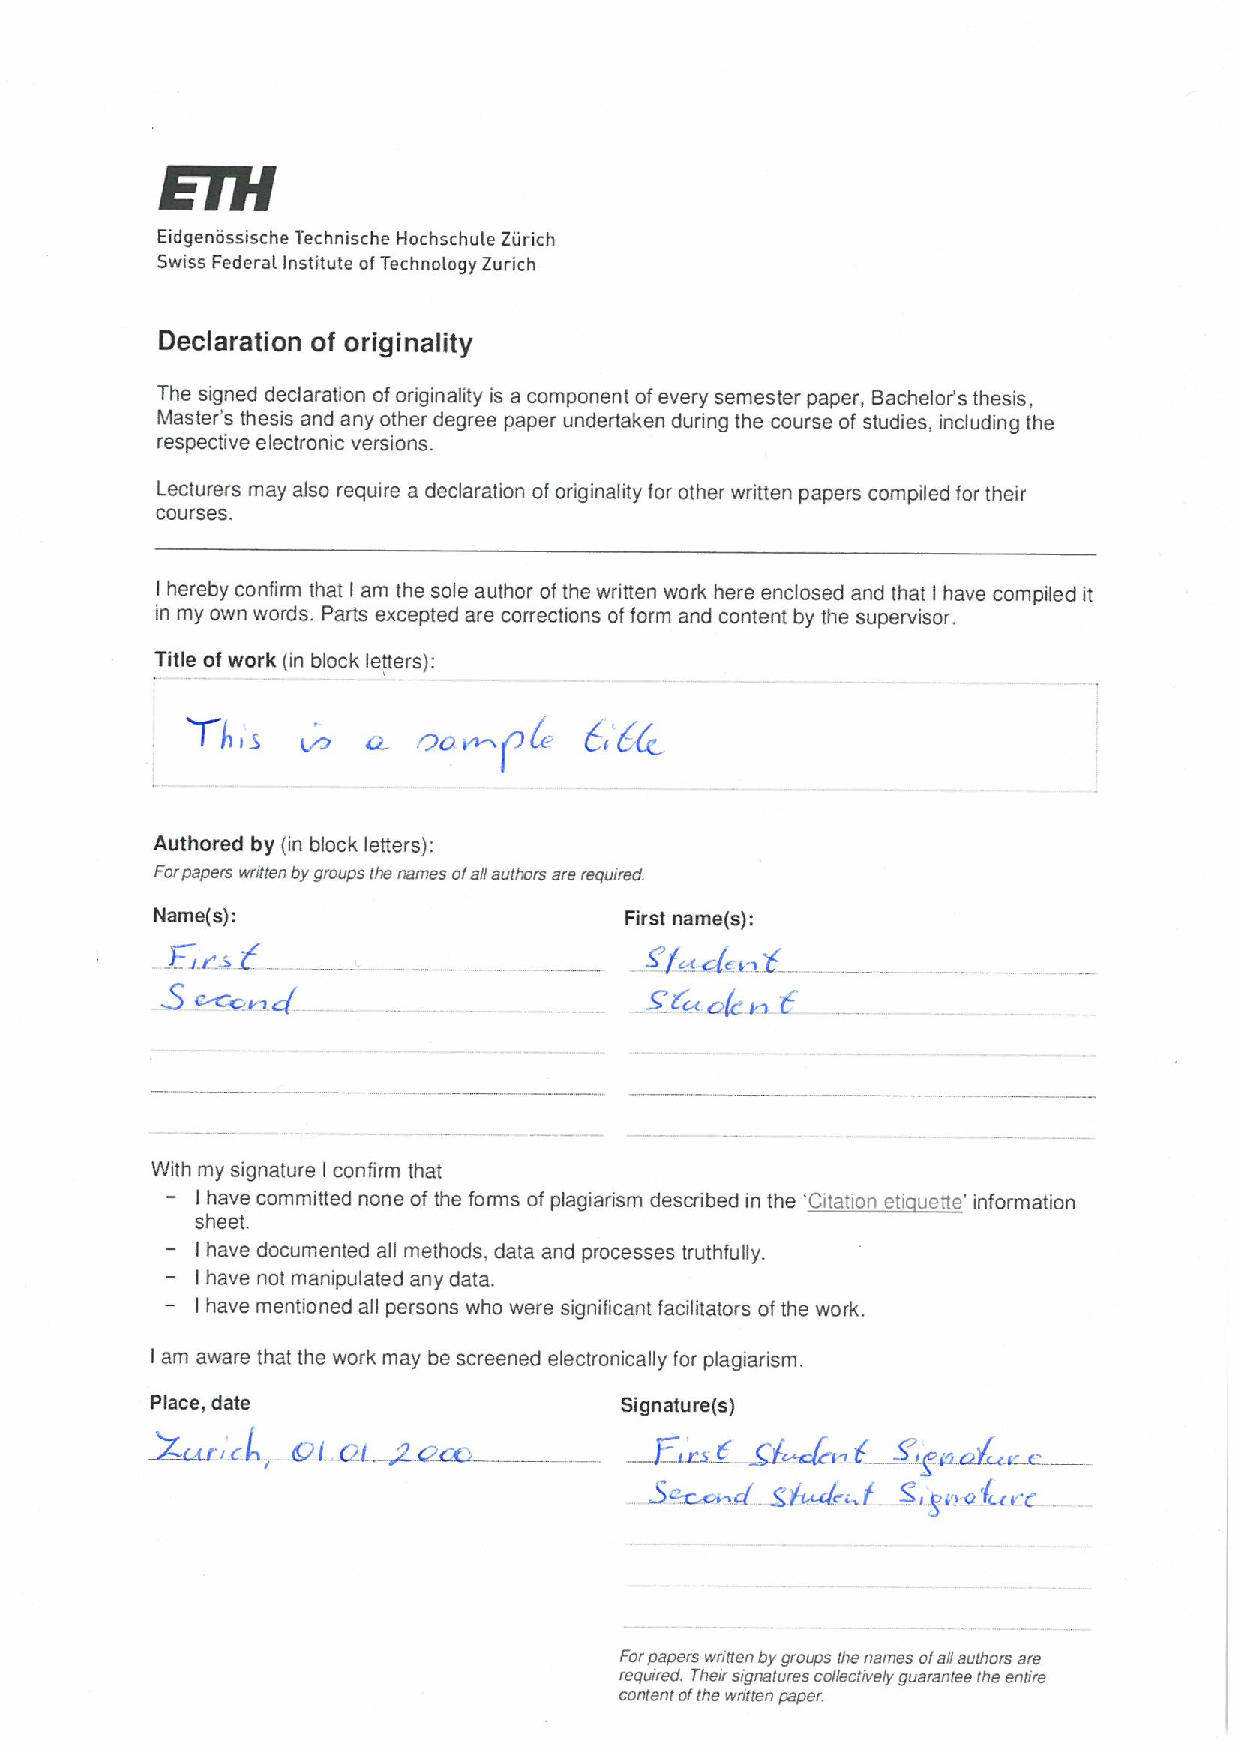
\includepdf[pages=-, turn=false, scale=0.9]{./figures/declaration_of_originality}


\chapter{File Structure}
Describe how the project directories/files are organized, e.g.:

\begin{flushleft}
\dirtree{%
.1 /.
  .2 README \DTcomment{A README with some general information about the project.}.
  .2 01\_report \DTcomment{The source files of the project report.}.
  .2 02\_presentation \DTcomment{The source files of the presentation.}.
  .2 03\_designflow \DTcomment{Some designflow-specific files.}.
}
\end{flushleft}

What needs to be done to run an RTL simulation (stimuli generation,
compilation...)?


\chapter{Datasets}
If you have a data set comprising several test images, you could
depict and describe them here. Use a simple naming scheme such that
you can easily refer to certain elements of this data set in the text.


\chapter{More Evaluation Results}
If you conducted an extensive evaluation you could move surplus
graphs/results to the appendix.


\chapter{Algorithms / Tables}
Large algorithm boxes and tables may clutter your chapters and impair
the readability. If they are not very important, consider moving them
to the appendix as well.


\chapter{ASIC Datasheet ($<$Chipname$>$)}

If you have designed an \gls{asic} during your work, you should
include a datasheet for your chip into the report. As soon as you
start testing your fabricated chip, you will be glad to have such a
datasheet. An example structure of such a datasheet is given in the
following. For more inspirations on what you may include in your
datasheet, have a look at the datasheet of a commercial \gls{ic}.

\minitoc

\section{Features}
\begin{itemize}
\item Lorem ipsum dolor sit amet, ...
\item Lorem ipsum dolor sit amet, ...
\item Lorem ipsum dolor sit amet, ...
\item Lorem ipsum dolor sit amet, ...
\end{itemize}

\section{Applications}
\lipsum[2]

\section{Description}
\lipsum[2]

\section{Packaging}
\lipsum[2]

\section{Bonding Diagram}
\lipsum[2]

\begin{figure}[htbp]
  \centering 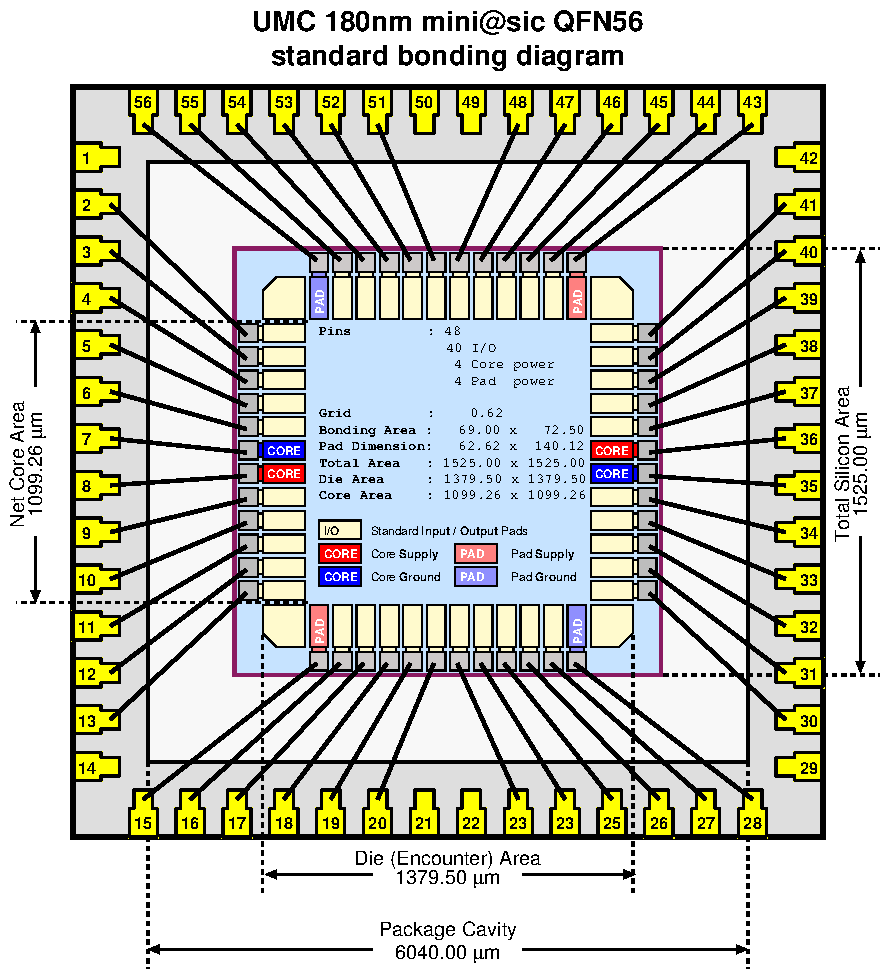
\includegraphics[width=0.9\textwidth]{./figures/qfn56_180_std}
  \caption{Bonding diagram.}
\end{figure}

\section{Pin Map}
\lipsum[2]

\begin{figure}[htbp]
  \centering 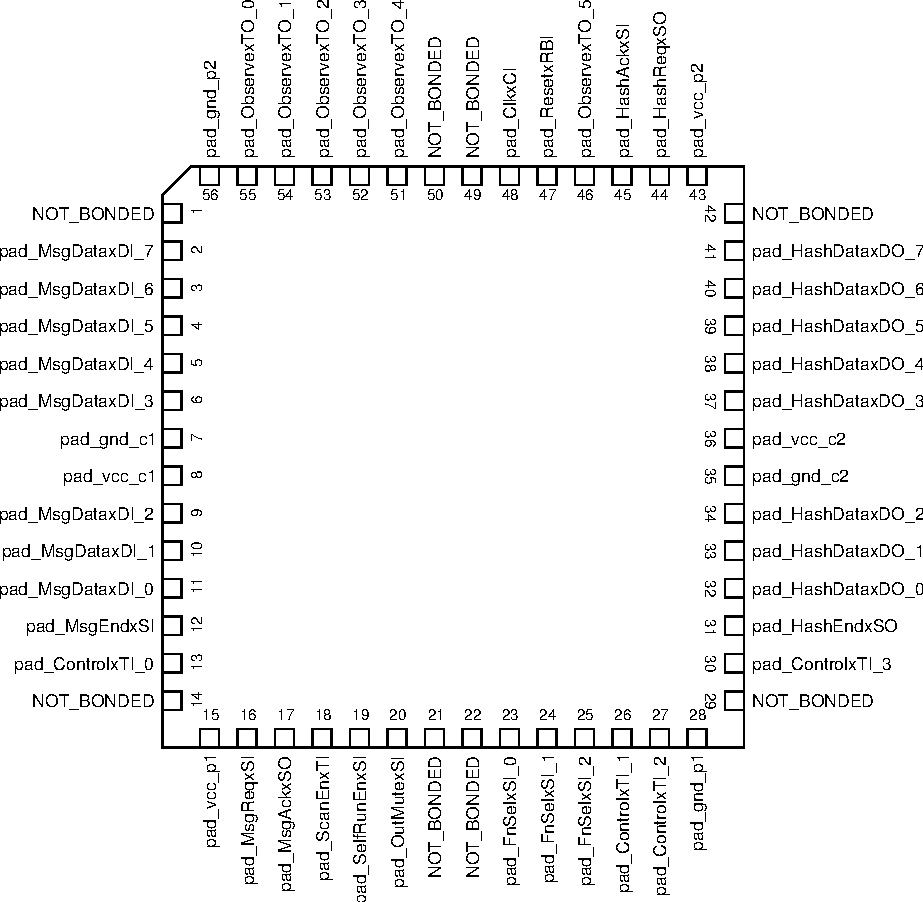
\includegraphics[width=1.0\textwidth]{./figures/asic_pinout}
  \caption{$<$Chipname$>$ pinout.}
\end{figure}

\section{Pin Description}
\lipsum[2]

\section{Interface Description}
\lipsum[2]

\section{Register Map}
\lipsum[2]

\section{Operation Modes}
\lipsum[2]

\subsection{Functional Modes}
\subsection{Test Modes}

\section{Electrical Specifications}
\lipsum[2]
\subsection{Recommended Operating Regions}
\subsection{Absolute Maximum Ratings}

%%%%%%%%%%%%%%%%%%%%%%%%%%%%%%%%%%%%%%%%%%%%%%%%%%%%%%%%%%%%%%%%%%%%%%%
%%%%%%%%%%%%%%%%%%%%%%%%%%%%%%%%%%%%%%%%%%%%%%%%%%%%%%%%%%%%%%%%%%%%%%%
%%%%%                                                                 %
%%%%%     z_02_directories.tex                                        %
%%%%%                                                                 %
%%%%% Author:      Michael Muehlberghuber (<mbgh@iis.ee.ethz.ch>      %
%%%%% Created:     01.07.2012                                         %
%%%%% Description: A description of all files and directories         %
%%%%%              contained within this LaTeX framework.             %
%%%%%                                                                 %
%%%%%                                                                 %
%%%%% History:                                                        %
%%%%%%%%%%%%%%                                                        %
%%%%%                                                                 %
%%%%% 01-Jul-2012 (Michael Muehlberghuber - mbgh@iis.ee.ethz.ch):     %
%%%%% *) Created initial version.                                     %
%%%%%                                                                 %
%%%%%%%%%%%%%%%%%%%%%%%%%%%%%%%%%%%%%%%%%%%%%%%%%%%%%%%%%%%%%%%%%%%%%%%
%%%%%%%%%%%%%%%%%%%%%%%%%%%%%%%%%%%%%%%%%%%%%%%%%%%%%%%%%%%%%%%%%%%%%%%

\chapter{The Template Directory Structure}

This \LaTeX{} framework suitable for creating reports spreads over
various directories and files. In order to give you a short overview
of this structure, the respective directories and the contained files
are described in the following:

\begin{flushleft}
\dirtree{%
.1 /.
  .2 README \DTcomment{README file with a quick start guide.}.
  .2 Makefile \DTcomment{Makefile with some \LaTeX{} related build targets.}.
  .2 report\_template.tex \DTcomment{The main \LaTeX{} file of the report document, which further loads other (content) files.}.
  .2 bib \DTcomment{Contains bibliography related files.}.
    .3 main.bib \DTcomment{Bibliography file.}.
  .2 content \DTcomment{Contains the actual source files of your report.}.
    .3 *$.$tex \DTcomment{Here, multiple content files are provided.}.
  .2 figures \DTcomment{Contains the images which are loaded during your report.}.
    .3 eth\_logo.* \DTcomment{ETH logo in \gls{eps} and \gls{pdf} format.}.
    .3 titlepage\_logo.* \DTcomment{Titlepage logo in \gls{eps} and \gls{pdf} format.}.
    .3 asic\_pinout.* \DTcomment{Sample pinout of an \gls{asic} in \gls{eps} and \gls{pdf} format.}.
  .2 figures\_raw \DTcomment{Contains the raw sources of your figures.}.
    .3 titlepage\_logo.obj \DTcomment{Tgif titlepage logo source.}.
  .2 glossaries \DTcomment{Contains glossaries.}.
    .3 glossaries.tex \DTcomment{The glossaries file containing both the entries of the list of acronym entries and the entries of the main glossary.}.
  .2 preamble \DTcomment{Contains preamble information of the document.}.
    .3 preamble.tex \DTcomment{Preamble of the report document.}.
}
\end{flushleft}


%%% Local Variables: 
%%% mode: latex
%%% TeX-master: "../report_template"
%%% End: 

%%%%%%%%%%%%%%%%%%%%%%%%%%%%%%%%%%%%%%%%%%%%%%%%%%%%%%%%%%%%%%%%%%%%%%%
%%%%%%%%%%%%%%%%%%%%%%%%%%%%%%%%%%%%%%%%%%%%%%%%%%%%%%%%%%%%%%%%%%%%%%%
%%%%%                                                                 %
%%%%%     z_03_latex_tips.tex                                         %
%%%%%                                                                 %
%%%%% Author:      Michael Muehlberghuber (<mbgh@iis.ee.ethz.ch>      %
%%%%% Created:     01.07.2012                                         %
%%%%% Description: Some LaTeX-specific writing tips                   %
%%%%%                                                                 %
%%%%%                                                                 %
%%%%% History:                                                        %
%%%%%%%%%%%%%%                                                        %
%%%%%                                                                 %
%%%%% 01-Jul-2012 (Michael Muehlberghuber - mbgh@iis.ee.ethz.ch):     %
%%%%% *) Created initial version.                                     %
%%%%%                                                                 %
%%%%%%%%%%%%%%%%%%%%%%%%%%%%%%%%%%%%%%%%%%%%%%%%%%%%%%%%%%%%%%%%%%%%%%%
%%%%%%%%%%%%%%%%%%%%%%%%%%%%%%%%%%%%%%%%%%%%%%%%%%%%%%%%%%%%%%%%%%%%%%%

\chapter{\LaTeX{} Tips}

Writing a report with \LaTeX{} may not be as intuitive as it is the
case with \gls{wysiwyg} editors. Especially if you are using \LaTeX{}
(more or less) the first time, some problems with the syntax will
occur. In general, the present document should already serve as a good
starting point for your report and in the best case you only have to
insert the content of your project based on this framework.

Nevertheless, I will try to give some useful tips with regard to
\LaTeX{} throughout the next sections, which may help you to increase
the quality of your documents even further. If you want to use any of
the presented ideas, simply copy the \LaTeX{} source code of the
appropriate section to your on document and adapt it accordingly.


\section{Compiling a \LaTeX{} Document}
\label{sec:compiling}

Basically, either \shell{latex} or \shell{pdflatex} can be used in
order to generate the document output in \gls{dvi} or \gls{pdf}
format, respectively. Throughout this section I will solely use the
\shell{pdflatex} command for demonstration purposes (if you prefer a
DVI document, just replace the \shell{pdflatex} command by
\shell{latex}0).

Compiling a latex document at the \gls{iis} computers is, in general,
as simple as executing the following command in a UNIX terminal
window:

\begin{shellenv}
pdflatex <document_name>
\end{shellenv}

Currently\footnote{State: July 2012} a \TeX{} Live version from the
year 2008 is the default distribution at the \gls{iis}. In order to
use the present \LaTeX{} framework for your report, you have to use a
more up-to-date version of \TeX{} Live, because the framework uses
some \LaTeX{} packages which are not part of the 2008 version. I
suggest using the 2011 version of \TeX{} Live. The simplest way to
check that you can build the report template successfully, is by
executing:

\begin{shellenv}
pdflatex-2011 report_template.tex
\end{shellenv}

This should (re)generate the \gls{pdf} output of the report template,
i.e., the file you are currently reading through. If typing in the
\shell{-2011} postfix becomes annoying for you, you may add aliases
into your \file{.cshrc} as follows:

\begin{shellenv}
alias latex 'latex-2011'
alias pdflatex 'pdflatex-2011'
\end{shellenv}

If you also want to (re)build the glossaries (maybe you have added
some acronyms or the like), you have to compile your report together
with the glossaries as follows:

\begin{shellenv}
pdflatex-2011 your_report.tex
makeglossaries-2011 your_report
pdflatex-2011 your_report.tex
\end{shellenv}

Furthermore, when you modify the references of your report (within the
bibliography file), you also have to (re)run \textsc{Bib}\TeX{} in
order to update your bibliography, i.e.:

\begin{shellenv}
pdflatex-2011 your_report.tex
bibtex-2011 your_report
pdflatex-2011 your_report.tex
pdflatex-2011 your_report.tex
\end{shellenv}


\section{Figures}
\label{sec:figures}

In order to include an image into your report (as it has been done
within in the previous sample chapters), you may use the
\texttt{figure} floating environment. With that, \LaTeX{} will take
care of placing them nicely and you can focus on the actual content of
your document. Figure~\ref{fig:std_eth_logo} shows an example of how
to insert a single figure.

\begin{figure}[htbp]
 \centering
\includegraphics[width=0.4\linewidth]{./figures/eth_logo}
 \caption{Standard ETH logo.}
 \label{fig:std_eth_logo}
\end{figure}

If you want to place multiple figures side-by-side, you can do this
with the use of \texttt{minipages}. Figure~\ref{fig:left_eth_logo} and
\ref{fig:right_eth_logo} illustrates an example.

\begin{figure}[htbp]
 \begin{minipage}[t]{0.45\linewidth}
  \centering
\includegraphics[width=1.0\linewidth]{./figures/eth_logo}
  \caption{Left ETH logo.}
  \label{fig:left_eth_logo}
 \end{minipage}\hfill
 \begin{minipage}[t]{0.45\linewidth}
  \centering
\includegraphics[width=1.0\linewidth]{./figures/eth_logo}
  \caption{Right ETH logo.}
  \label{fig:right_eth_logo}
 \end{minipage}
\end{figure}

In order to create a single figure with multiple subfigures, you can
do this as presented in Figure~\ref{fig:eth_logo_sub}

\begin{figure}[htbp]
 \centering
 \subfloat[Left ETH logo.]{
\includegraphics[width=0.3\textwidth]{./figures/eth_logo}}\hfill
 \subfloat[Center ETH logo.]{
\includegraphics[width=0.3\textwidth]{./figures/eth_logo}}\hfill
 \subfloat[Right ETH logo.]{
\includegraphics[width=0.3\textwidth]{./figures/eth_logo}}
 \caption{Multiple ETH logos as subfigures.}
 \label{fig:eth_logo_sub}
\end{figure}


\section{Tables}
\label{sec:tables}

Tables in \LaTeX{} allow you to present your results quite
nicely. Table~\ref{tab:std_table} shows a standard table.

\begin{table}[htbp]
 \caption{Standard table.}
 \label{tab:std_table}
 \centering\begin{tabular}{@{}lcr@{}} \toprule
  \textbf{Row 1 - Column 1} & \textbf{Row 1 - Column 2} & \textbf{Row 1 - Column 3} \\ \midrule
  Row 2 - Column 1 & Row 2 - Column 2 & Row 2 - Column 3 \\
  Row 3 - Column 1 & Row 3 - Column 2 & Row 3 - Column 3 \\
  Row 4 - Column 1 & Row 4 - Column 2 & Row 4 - Column 3 \\ \bottomrule
 \end{tabular}
\end{table}

Sometimes you may want to add a table which stretches one of its
columns in order to reach the full width of the document. Such an
example is shown in Table~\ref{tab:stretched_table}.

\begin{table}[htbp]
 \caption{Stretched table.}
 \label{tab:stretched_table}
 \centering\begin{tabularx}{1.0\linewidth}{@{}Xcr@{}} \toprule
  \textbf{Row 1 - Column 1} & \textbf{Row 1 - Column 2} & \textbf{Row 1 - Column 3} \\ \midrule
  Row 2 - Column 1 & Row 2 - Column 2 & Row 2 - Column 3 \\
  Row 3 - Column 1 & Row 3 - Column 2 & Row 3 - Column 3 \\
  Row 4 - Column 1 & Row 4 - Column 2 & Row 4 - Column 3 \\ \bottomrule
 \end{tabularx}
\end{table}

If you need to place two tables next to each other, you may use an
approach based on \texttt{minipages} as shown in Table~\ref{tbl:left}
and Table~\ref{tbl:right}.

\begin{figure}
  \begin{minipage}{0.49\textwidth}
    \captionof{table}{Left table.}
    \label{tbl:left}
    \centering\begin{tabular}{@{}lr@{}} \toprule
      Row 1 - Column 1 & Row 1 - Column 2 \\ \midrule
      Row 2 - Column 1 & Row 2 - Column 2 \\
      Row 3 - Column 1 & Row 3 - Column 2 \\
      Row 4 - Column 1 & Row 4 - Column 2 \\ \bottomrule
    \end{tabular}
  \end{minipage} \hfill
  %
  \begin{minipage}{0.49\textwidth}
    \captionof{table}{Right table.}
    \label{tbl:right}
    \centering\begin{tabular}{@{}lr@{}} \toprule
      Row 1 - Column 1 & Row 1 - Column 2 \\ \midrule
      Row 2 - Column 1 & Row 2 - Column 2 \\
      Row 3 - Column 1 & Row 3 - Column 2 \\
      Row 4 - Column 1 & Row 4 - Column 2 \\ \bottomrule
    \end{tabular}
  \end{minipage}
\end{figure}

\section{Creating Glossaries}

In order to generate a glossary within your report (e.g., a list of
acronyms or an actual glossary), take a look into the file
\texttt{glossaries.tex}. There, you will find some examples on how to
define an acronym as well as a glossary entry. If you want to
reference one of the acronyms within your report, you can do it the
same way as I did it with the \gls{led} right here (just take a look
into the source code).

As already mentioned in Section~\ref{sec:compiling}, you have to
rebuild your glossaries in order to display changes. For that, you
first have to build your document using \texttt{latex-2011} or
\texttt{pdflatex-2011} in a shell window, or the \textit{build-button}
in your preferred \LaTeX{} editor GUI. Next, you have to call
\texttt{makeglossaries-2011 \parameter{file\_name}} in a shell
window\footnote{The \texttt{makeglossaries} script is a Perl script
  available at the IIS computer system and should also be part of most
  \TeX{} distributions.}, followed by another build process of your
main source file, i.e.:

\begin{shellenv}
pdflatex-2011 your_report.tex
makeglossaries-2011 your_report
pdflatex-2011 your_report.tex
\end{shellenv}


\section{Creating Algorithm Boxes}

Algorithm boxes in \LaTeX{} allow you to present your algorithms in
pseudo code as shown in the following example:

\begin{algorithm}
  \SetKwData{Left}{left}\SetKwData{This}{this}\SetKwData{Up}{up}
  \SetKwFunction{Union}{Union}\SetKwFunction{FindCompress}{FindCompress}
  \SetKwInOut{Input}{input}\SetKwInOut{Output}{output}

  \Input{A bitmap $Im$ of size $w\times l$}
  \Output{A partition of the bitmap}
  \BlankLine
  \emph{special treatment of the first line}\;
  \For{$i\leftarrow 2$ \KwTo $l$}{
    \emph{special treatment of the first element of line $i$}\;
    \For{$j\leftarrow 2$ \KwTo $w$}{\label{forins}
      \Left$\leftarrow$ \FindCompress{$Im[i,j-1]$}\;
      \Up$\leftarrow$ \FindCompress{$Im[i-1,]$}\;
      \This$\leftarrow$ \FindCompress{$Im[i,j]$}\;
      \If(\tcp*[h]{O(\Left,\This)==1}){\Left compatible with \This}{\label{lt}
        \lIf{\Left $<$ \This}{\Union{\Left,\This}}\;
        \lElse{\Union{\This,\Left}\;}
      }
      \If(\tcp*[f]{O(\Up,\This)==1}){\Up compatible with \This}{\label{ut}
        \lIf{\Up $<$ \This}{\Union{\Up,\This}}\;
        \tcp{\This is put under \Up to keep tree as flat as possible}\label{cmt}
        \lElse{\Union{\This,\Up}}\tcp*[r]{\This linked to \Up}\label{lelse}
      }
    }
    \lForEach{element $e$ of the line $i$}{\FindCompress{p}}
  }
  \caption{disjoint decomposition}\label{algo_disjdecomp}
\end{algorithm}


% \section{Citing}


% \section{Units}

%%% Local Variables:
%%% mode: latex
%%% TeX-master: "../report_template"
%%% End:

%%%%%%%%%%%%%%%%%%%%%%%%%%%%%%%%%%%%%%%%%%%%%%%%%%%%%%%%%%%%%%%%%%%%%%%
%%%%%%%%%%%%%%%%%%%%%%%%%%%%%%%%%%%%%%%%%%%%%%%%%%%%%%%%%%%%%%%%%%%%%%%
%%%%%                                                                 %
%%%%%     z_04_writing_tips.tex                                       %
%%%%%                                                                 %
%%%%% Author:      Michael Muehlberghuber (<mbgh@iis.ee.ethz.ch>      %
%%%%% Created:     01.07.2012                                         %
%%%%% Description: Some Writing-specific tips in general.             %
%%%%%                                                                 %
%%%%% History:                                                        %
%%%%%%%%%%%%%%                                                        %
%%%%%                                                                 %
%%%%% 01-Jul-2012 (Michael Muehlberghuber - mbgh@iis.ee.ethz.ch):     %
%%%%% *) Created initial version.                                     %
%%%%%                                                                 %
%%%%%%%%%%%%%%%%%%%%%%%%%%%%%%%%%%%%%%%%%%%%%%%%%%%%%%%%%%%%%%%%%%%%%%%
%%%%%%%%%%%%%%%%%%%%%%%%%%%%%%%%%%%%%%%%%%%%%%%%%%%%%%%%%%%%%%%%%%%%%%%

\chapter{General Writing Guidelines}

As soon as you get familiar with the syntax of \LaTeX{} (and I can
promise you, you will get familiar with it quite quickly as soon as
you start writing your reports with \LaTeX{}), some more general
writing tips might become of interest for your. Therefore, I collected
a few general writing guidlines in the following sections, some of
them with regard to \LaTeX{}, some of them not.

\paragraph{Placement of Floating Environments}
Figures and tables are the two most prominent examples for floating
environments. Although the figure examples presented in
Section~\ref{sec:figures} use \texttt{[htbp]} to tell \LaTeX{} how to
place them, you should normally only use the \texttt{h} parameter if
you really require it. Since \LaTeX{} then at first tries to place the
figure at the same position as its source code, this somehow
contradicts with the actual purpose of the \texttt{figure}
environment. So, in general, try to place floating environments using
one of the following parameters:

\begin{description}
\item[t] Place the floating environment on \textbf{t}op of a page.
\item[b] Place the floating environment on the \textbf{b}ottom of a
  page.
\item[p] Puts the floating environment on a single \textit{floating
    \textbf{p}age} with other floating environments.
\end{description}


\paragraph{Positioning of Figure and Table Captions}
Captions of figures are, in general, placed below the actual figure,
whereas captions of tables should be placed on top of
them. Section~\ref{sec:figures} and \ref{sec:tables} contain some
examples for figures and tables, including correct placement of
captions.


\paragraph{Avoid Unneccessary \LaTeX{} Packages}
Although there are so many ``cool'' \LaTeX{} packages available
everywhere on the Internet, try to use only those, which you really
require. The main problem with loading too many, more or less unknown,
packages is that some of them might redefine some commands, etc.,
which are used by another package which asumes that command to be the
original one. Keeping track of these changes and the relations between
different packages, is quite annoying and takes quite a lot of
time. Hence, keep your preamble simple with regard to packages.


\paragraph{Make Use of Vector Drawings}
Since \LaTeX{} handles vector drawings pretty good and their
scalability allows you to print them in any resolution, prefer them
compared to their pixel counterparts and use them whenever possible.

% \paragraph{Equations Within the ``Text-Flow''}

% \paragraph{Punctuation within Captions}
% \begin{itemize}
%  \item No second fullstop when ending sentences with abbreviations like
%  etc.
% \end{itemize}

%%% Local Variables:
%%% mode: latex
%%% TeX-master: "../report_template"
%%% End:


\backmatter

% Print the main glossary.
\printglossary[type=main,title=Glossary]


% Print the bibliography.
\nocite*{} % Print non-cited references as well.
\bibliographystyle{IEEEtran}
\bibliography{IEEEabrv,./bib/main}


\end{document}
%%%%%%%%%%%%%%%%%%%%%%%%%%%%%%%%%%%%%%%%%%%%%%%%%%%%%%%%%%%%%%%%%%%%%%%
%%%%%                                                                 %
%%%%%     End of Document                                             %
%%%%%                                                                 %
%%%%%%%%%%%%%%%%%%%%%%%%%%%%%%%%%%%%%%%%%%%%%%%%%%%%%%%%%%%%%%%%%%%%%%%
